% #region PREAMBEL OG PAKKER
\documentclass[a4paper, 12pt]{article}  % DOKUMENTKLASSE
\title{IIK3100 -- Etisk hacking og penetrasjonstesting\\[0.25em]Home Exam}               % TITTEL
\author{Håvard Solberg Nybøe}           % FORFATTER
\date{\today}                    % DATO & FAG

\usepackage[english]{babel}      % NORSK SPRÅK
\usepackage[
    backend=biber,style=apa]{biblatex}  % BIBLIOGRAFI
\usepackage{csquotes}                   % PAKKE TIL BABEL
\addbibresource{bibliografi.bib}        % PATH TIL BIBLIOGRAFI
\usepackage[hidelinks]{hyperref}        % LENKER I TOC OG GENERELT
\usepackage[margin=1in]{geometry}       % VANLIG STØRRELSE MARGIN
\setlength{\parindent}{0em}             % SKILLER AVSNITT
\usepackage{graphicx}                   % BILDER \includegraphics[OPTIONS]{PATH}
\usepackage{kantlipsum}                 % FYLLTEKST I KANT-STIL (kant[n-m])
\usepackage{amsfonts,                   % BLACKBOARD BOLD FONT (\mathbb{N})
amsmath,stmaryrd,amssymb}         % ANDRE MATTE PAKKER
\usepackage{caption}                    % PAKKE FOR BEDRE CAPTIONS I FIGURER
\usepackage{float}                      % FLYTT FIGURER 
% #endregion
% \includeonly{sections/web-hacking}
\begin{document}

\setlength{\parskip}{0em}             % LINJEAVSTAND
\maketitle
\tableofcontents % INNHOLDSFORTEGNELSE
\setlength{\parskip}{.8em}             % LINJEAVSTAND

\section{OSINT}
\newpage
\section{Technical Information Gathering}

\subsection{Vipps backoffice (30p)}
Can you find the backoffice website of Vipps? Send the domain as a flag!

\textbf{Solution:}\\
The difficulty in this task was mostly finding a website that could look for and display subdomains without a paywall, since my manual attempts at finding the subdomain failed. I found a website called pentest-tools.com that could do this for me.

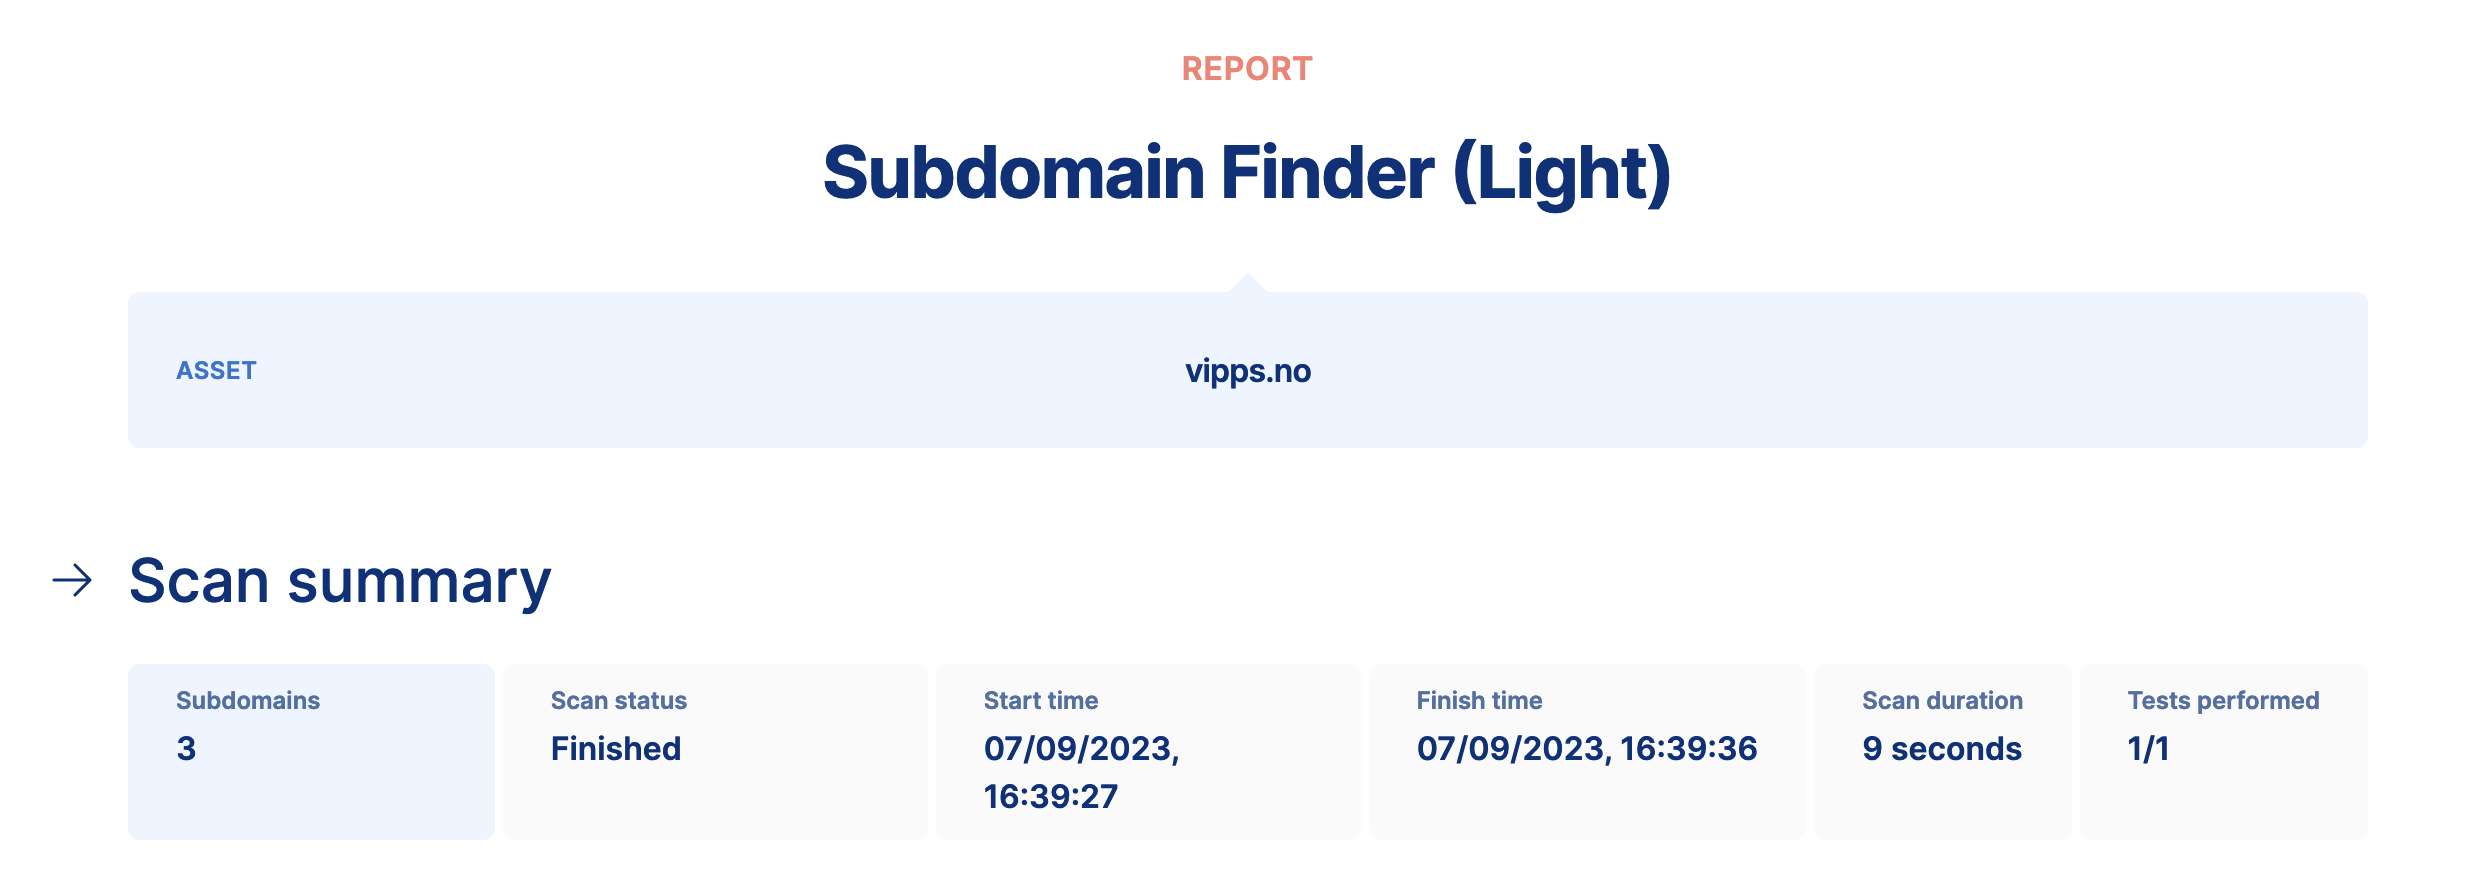
\includegraphics[width=15cm]{img/Technical information gathering/Vipps Backoffice/Skjermbilde 2023-09-07 kl. 15.40.23.png}

After the scan three subdomains were found, and the one that looked most promising was backoffice-test.vipps.no.

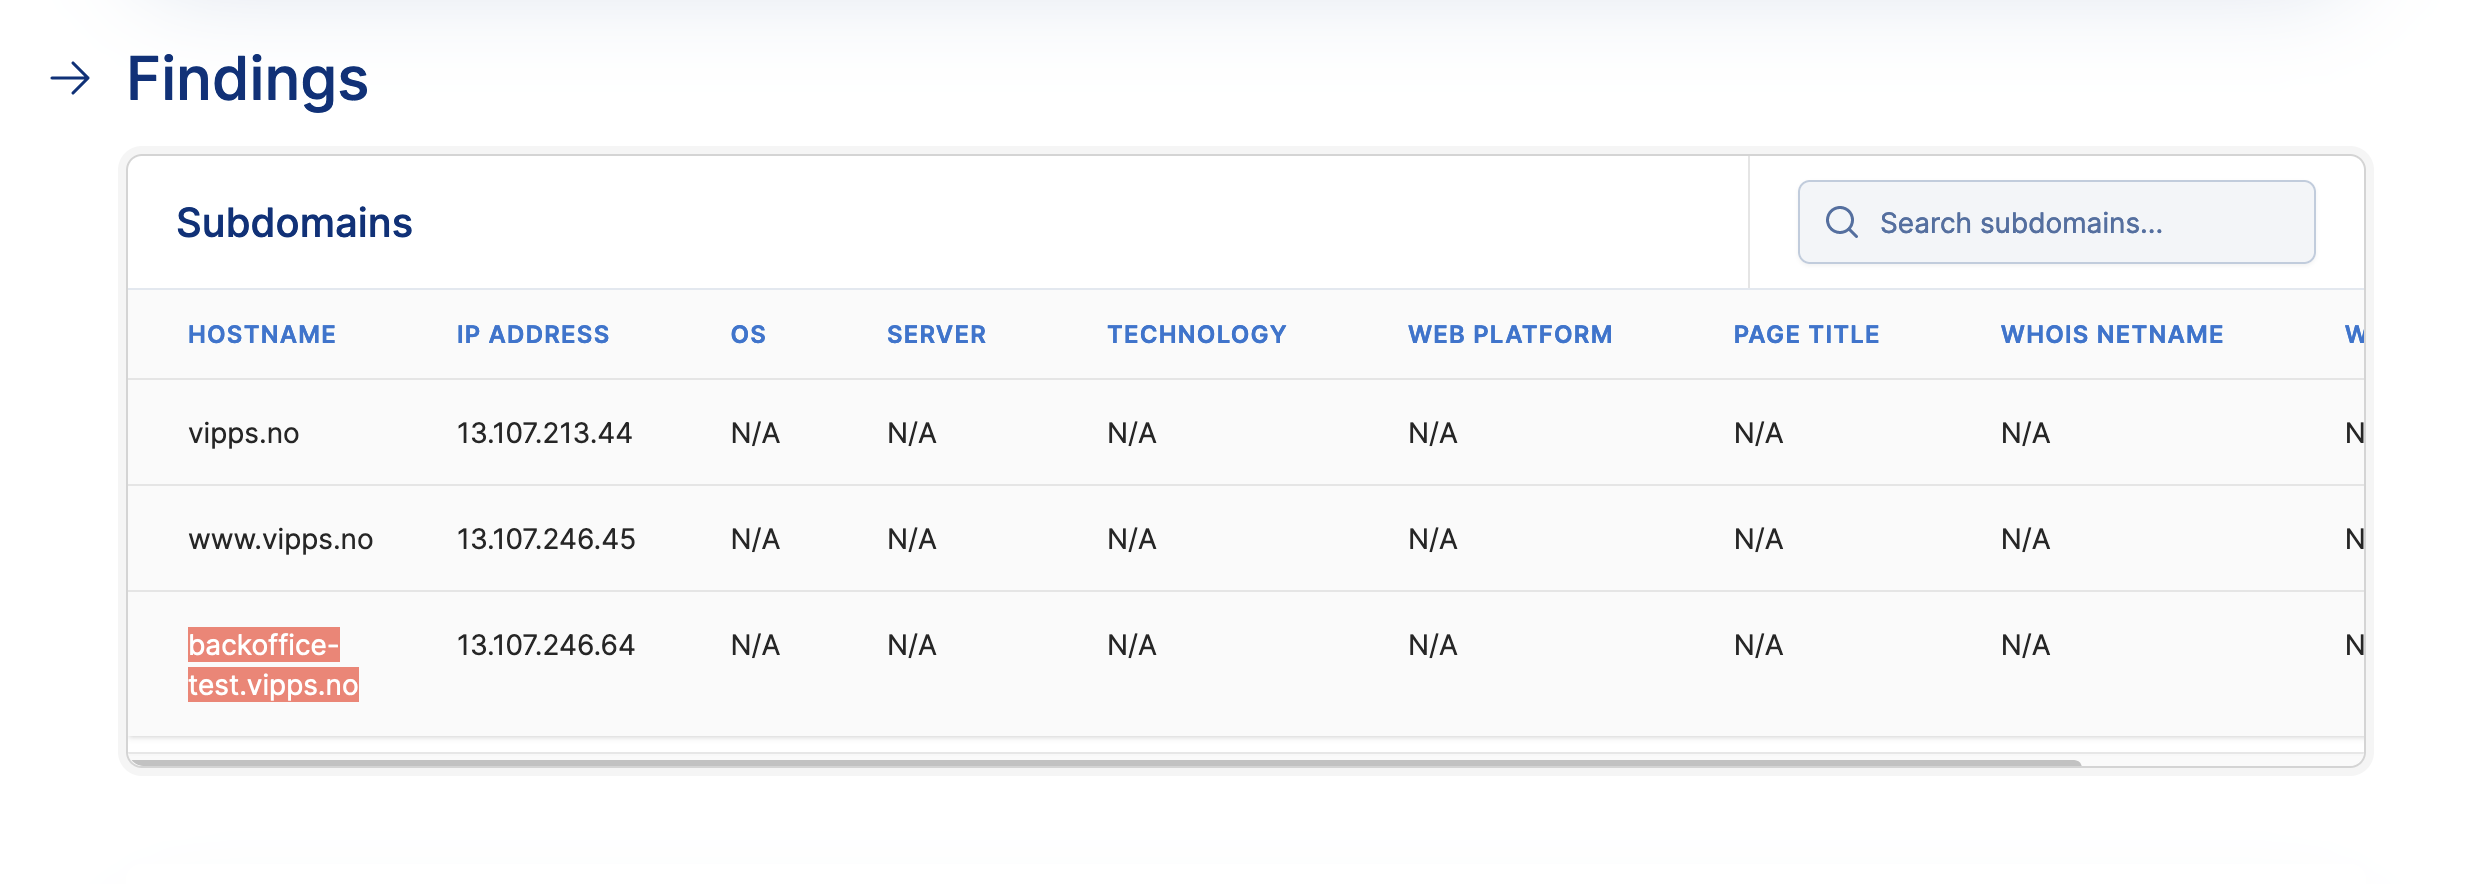
\includegraphics[width=15cm]{img/Technical information gathering/Vipps Backoffice/Skjermbilde 2023-09-07 kl. 15.40.13.png}

\newpage
\subsection{Vy (30p)}
Find the network range of Vy in Norway! Write it in CIDR format!

\textbf{Solution:}\\
This task was pretty straight forward, all I needed to di was look up vy.no on dnsdumpster.com.

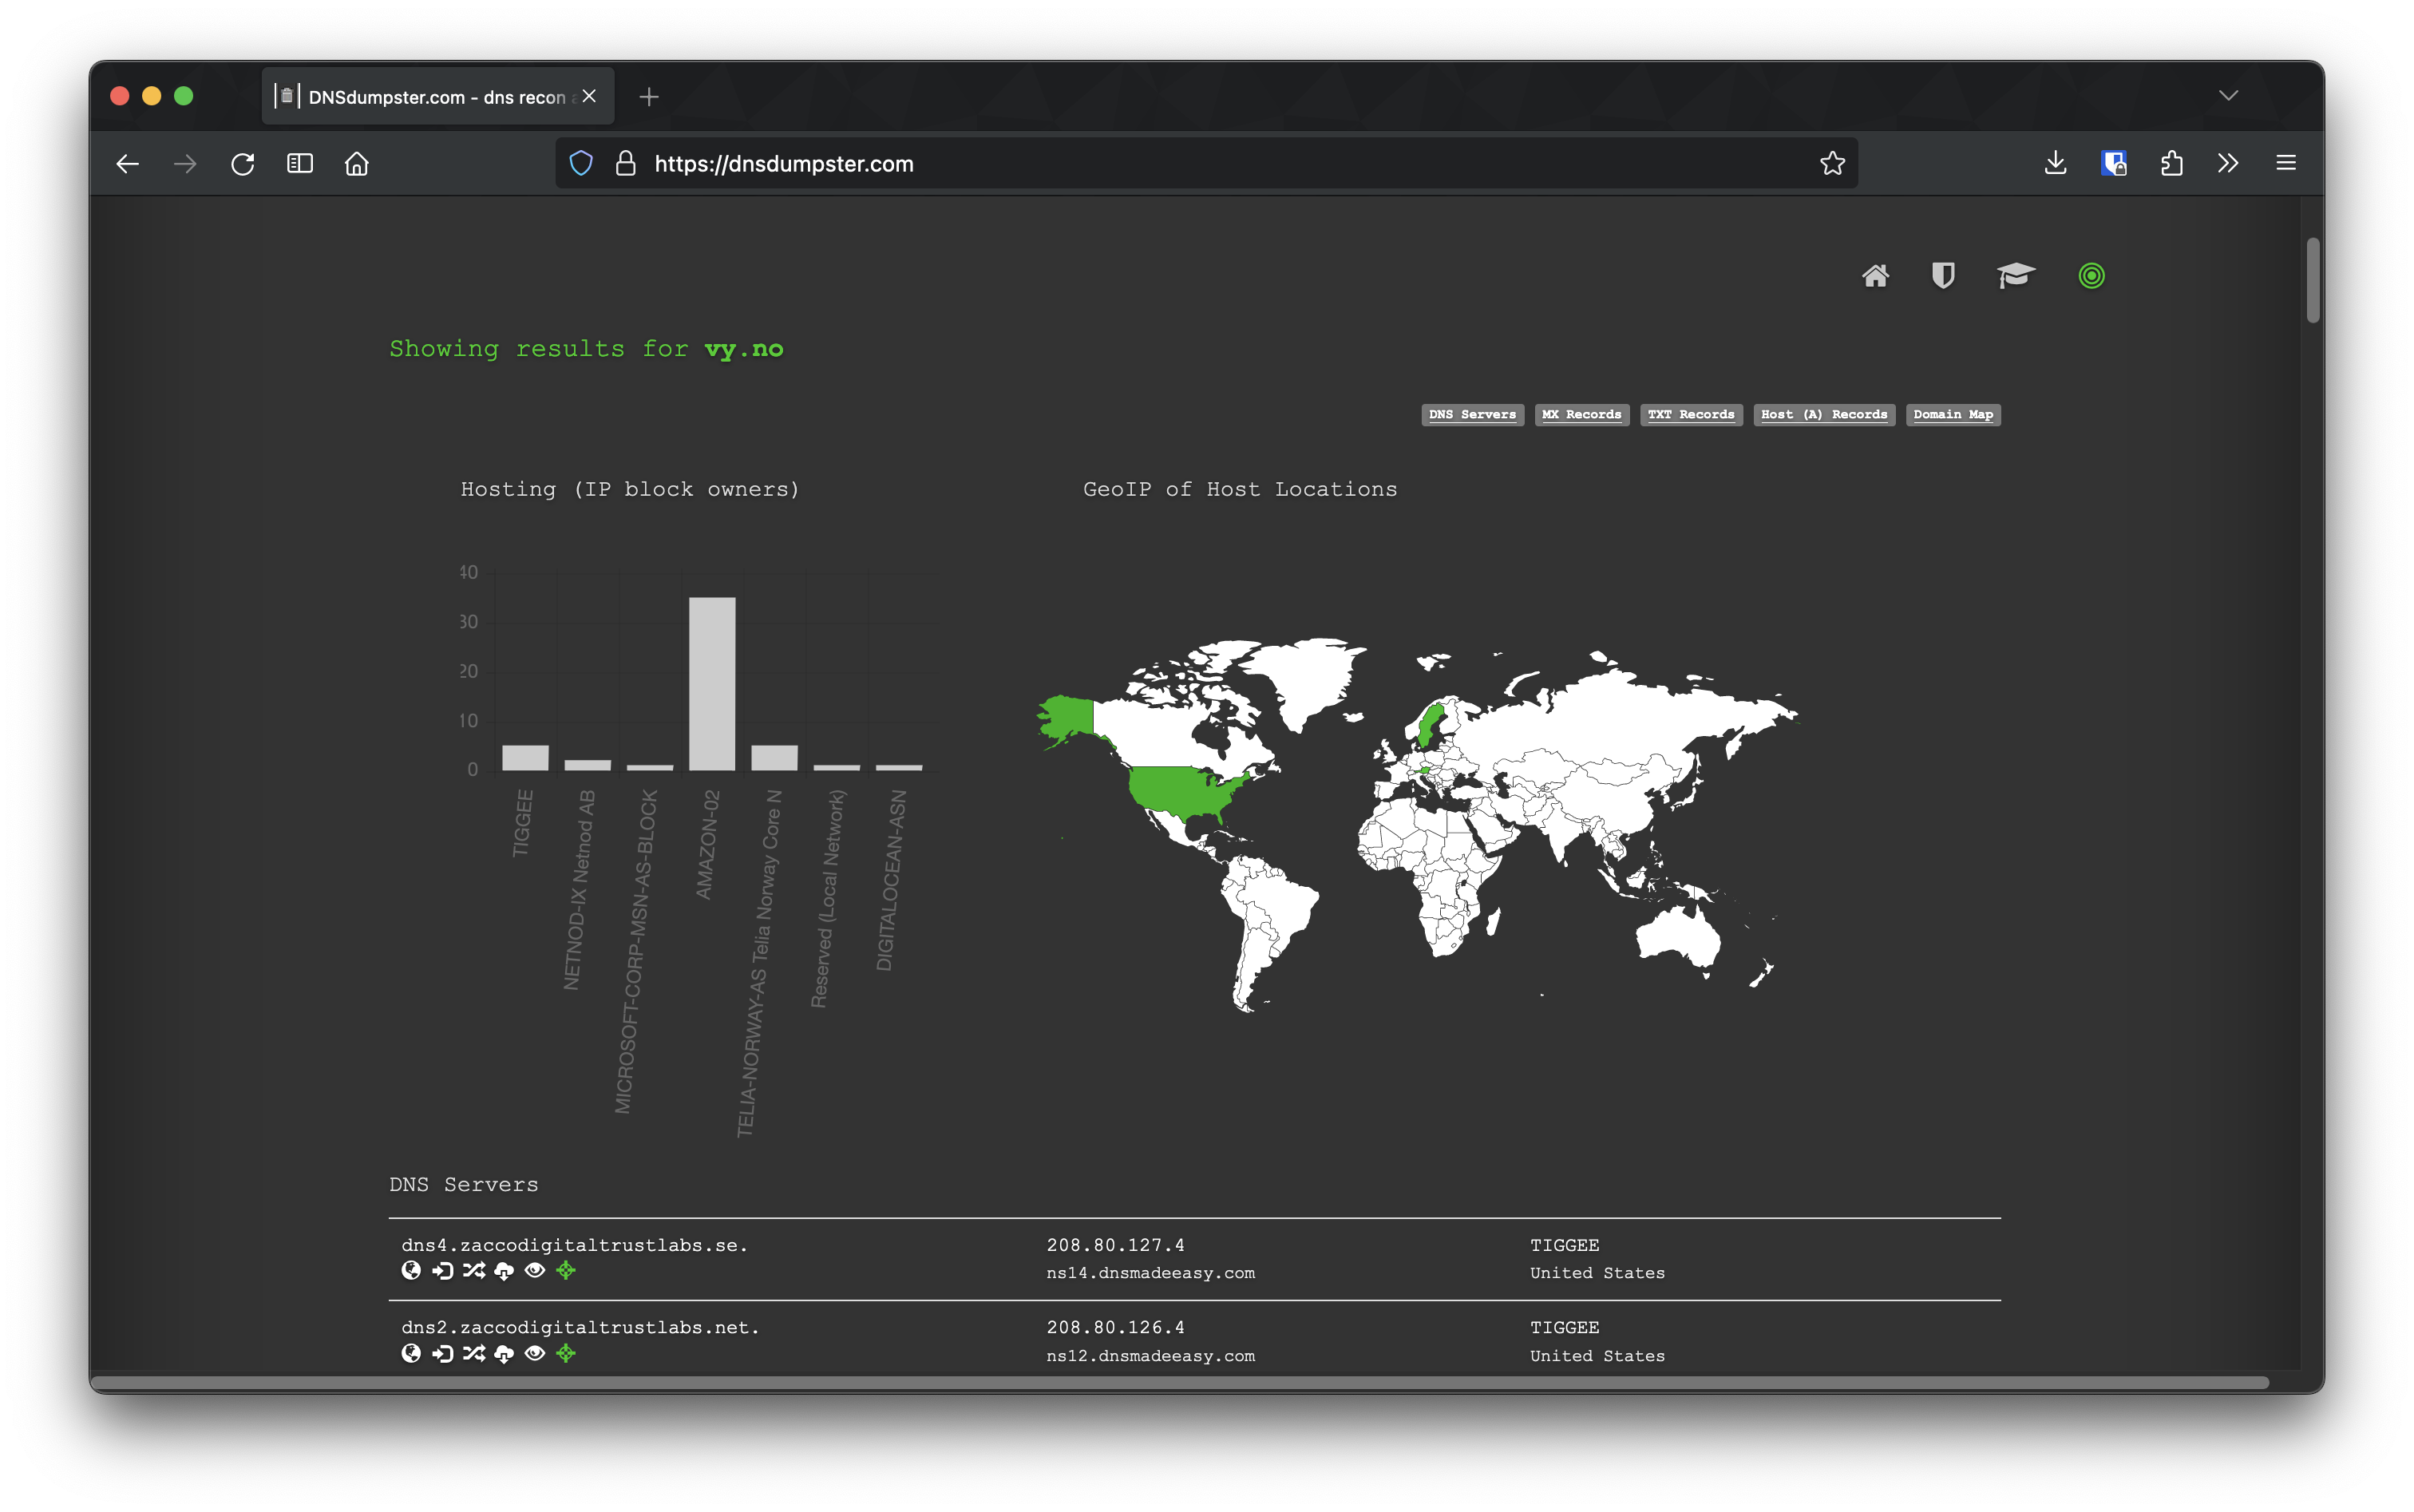
\includegraphics[width=15cm]{img/Technical information gathering/Vy/Skjermbilde 2023-09-01 kl. 14.56.00.png}

Then find an IP-address from Norway\dots

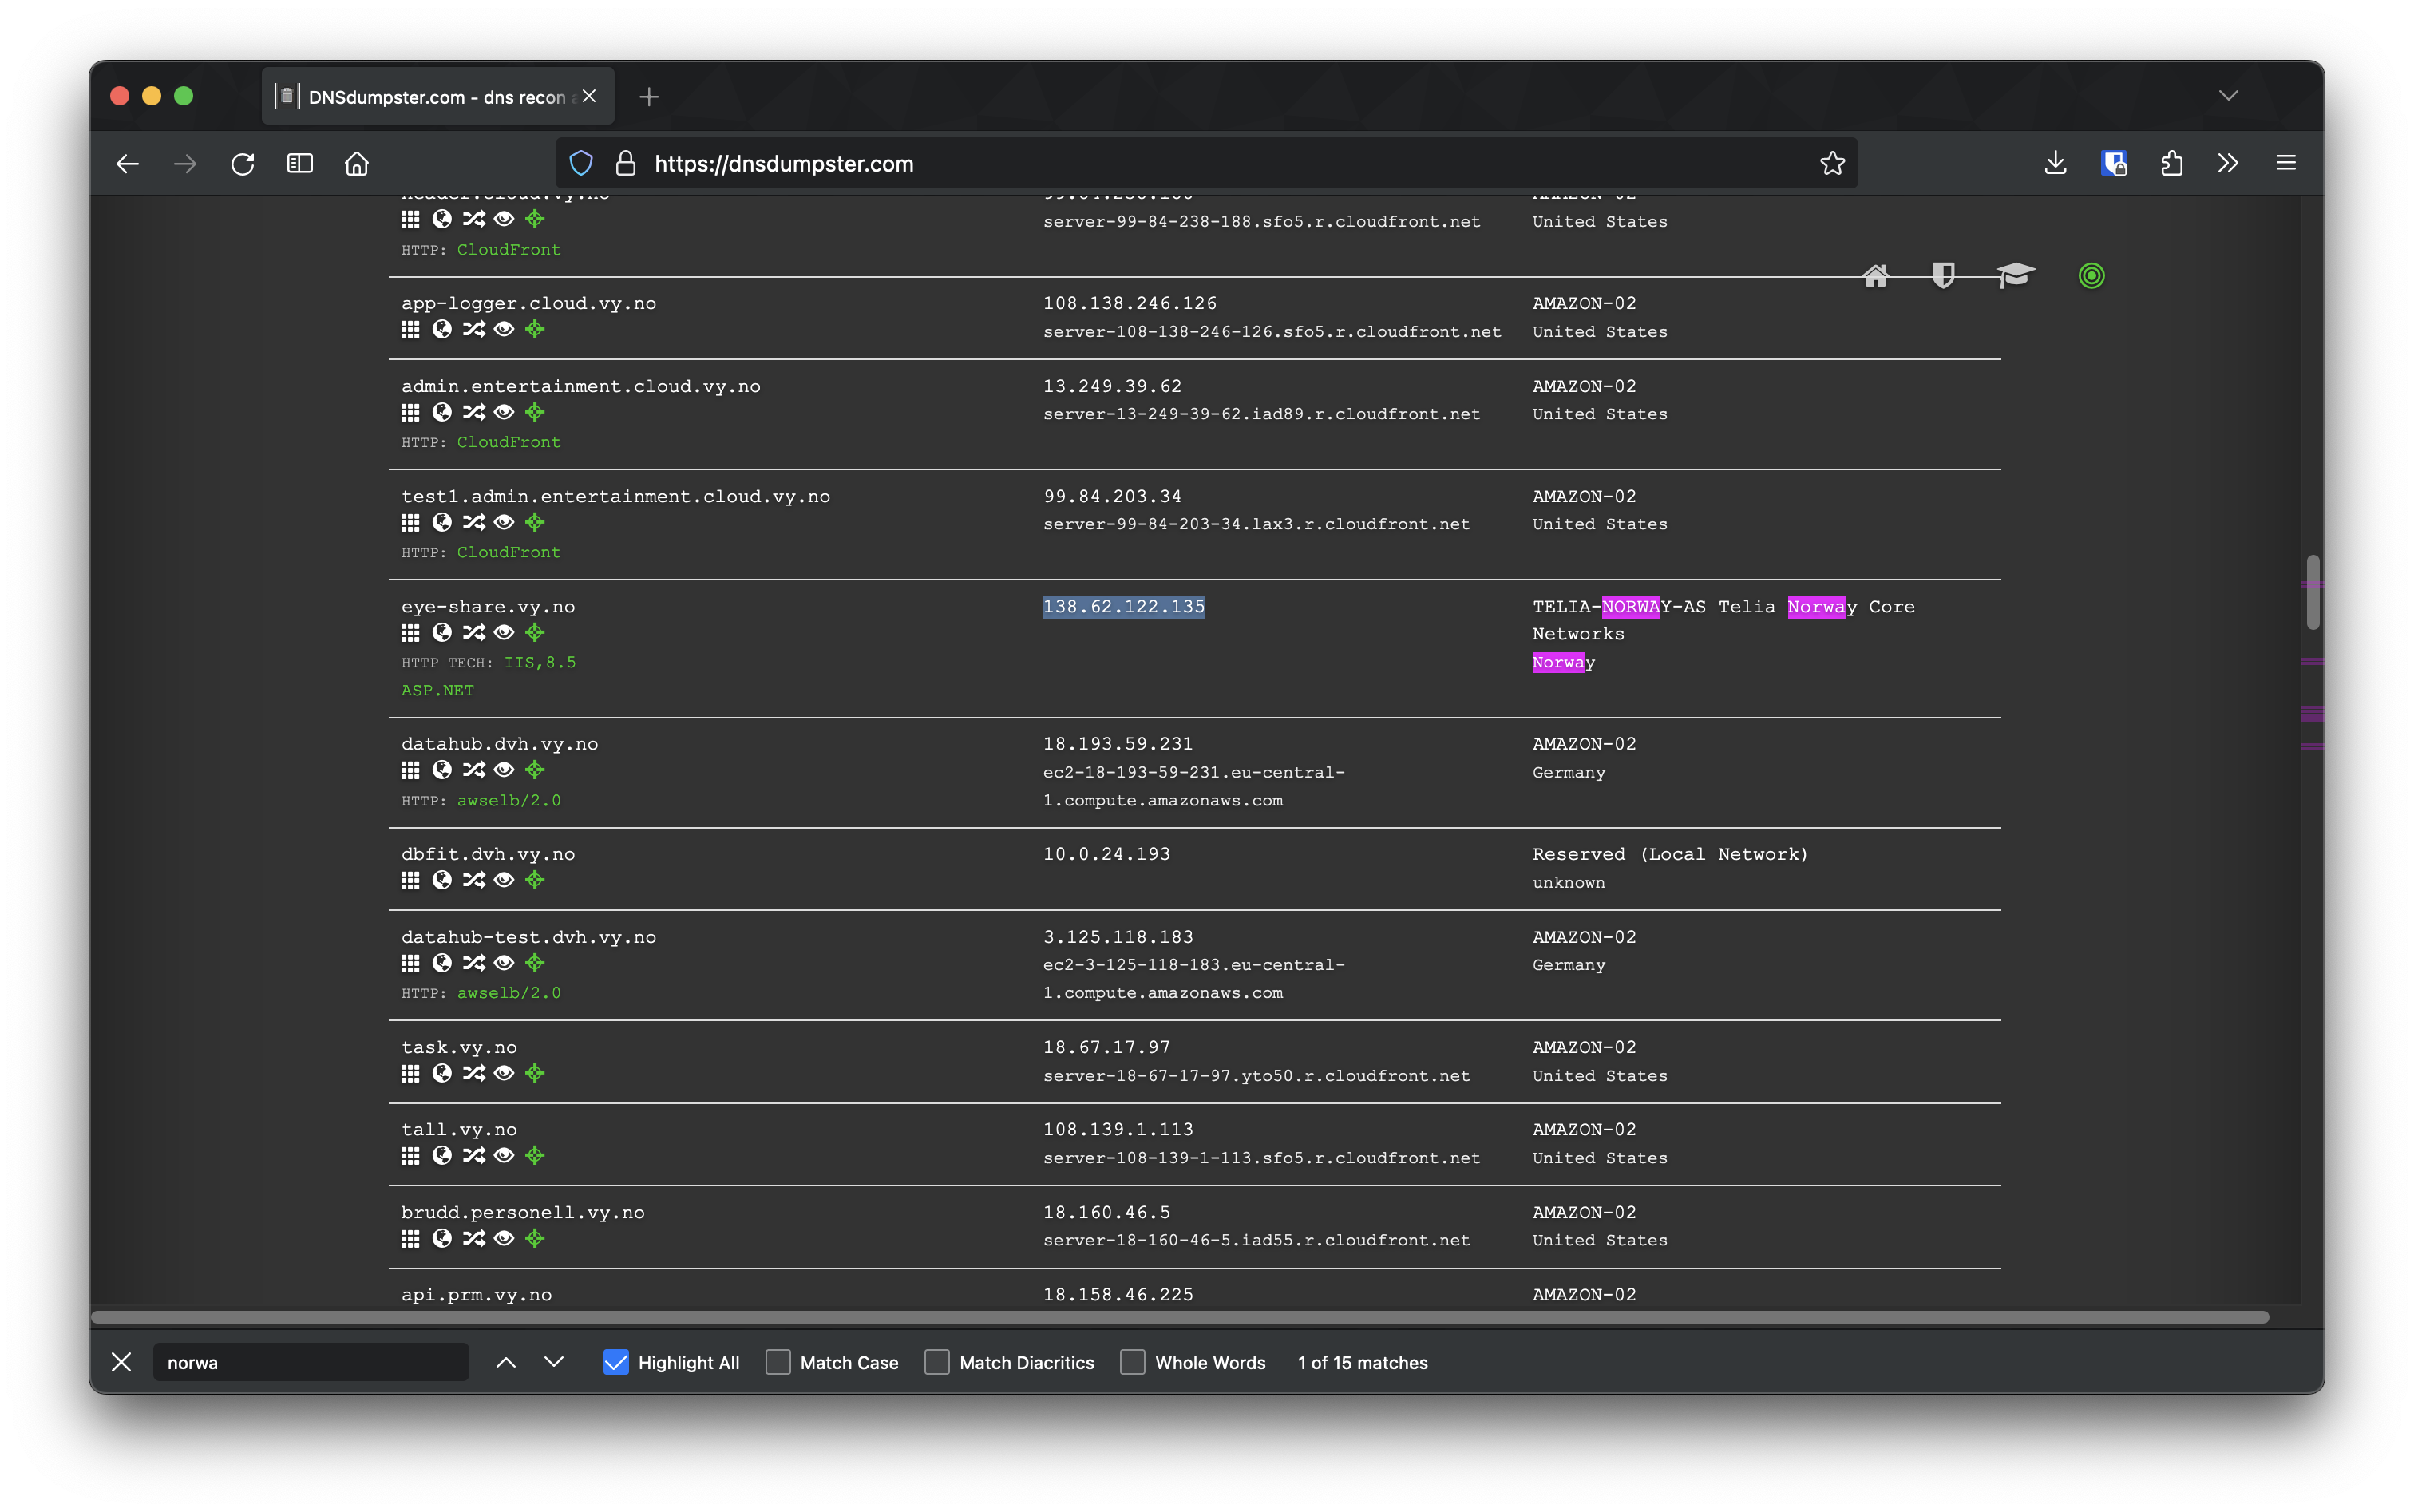
\includegraphics[width=15cm]{img/Technical information gathering/Vy/Skjermbilde 2023-09-01 kl. 14.56.23.png}

\dots and look it up in the RIPE database.

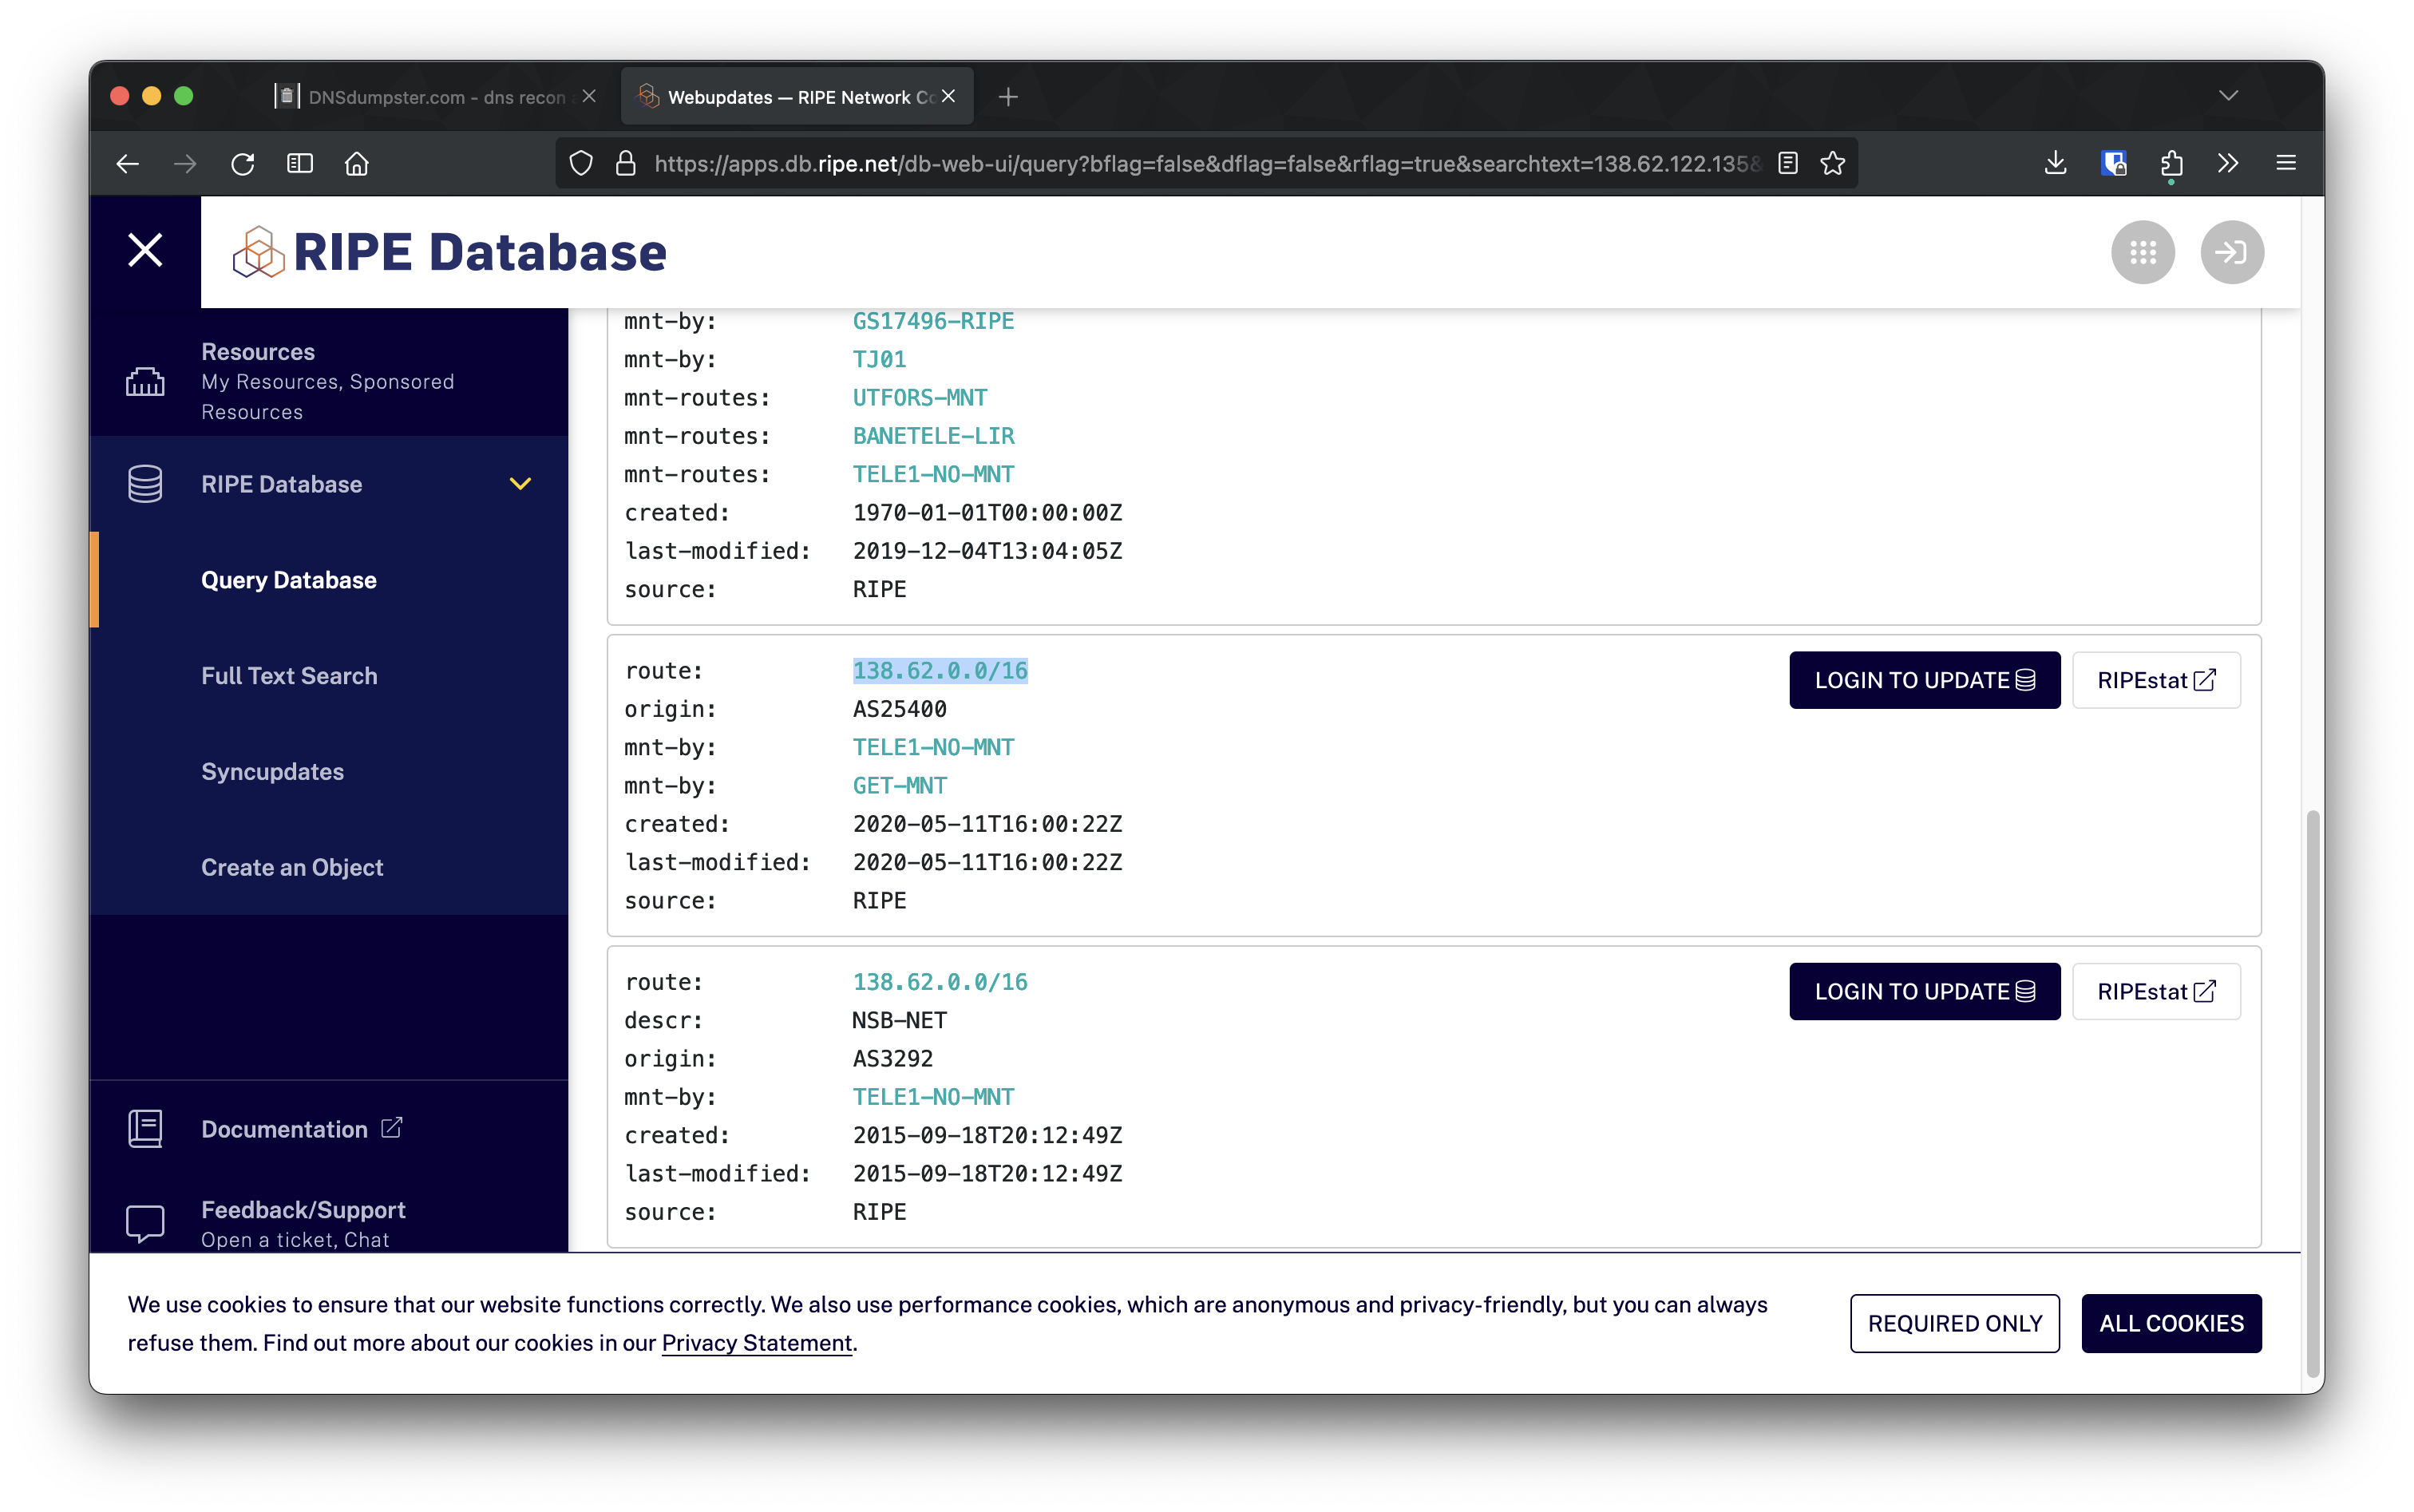
\includegraphics[width=15cm]{img/Technical information gathering/Vy/Skjermbilde 2023-09-01 kl. 14.56.50.png}
\section{Network Mapping}

\section{Get In Touch With Services}

\subsection{Casanova (70p)}
My service is running on \texttt{kenobi.hackingarena.com}, port \texttt{9393}. My name is Casanova (username: \texttt{casanova}). I have a huge problem. One of my exgirlfriends somehow figured out my password and want to realese all details about my affairs. How she figured it out??? I was so cautios. Ok, I'm using the same password everywhere, but I never had any incident (except for this emberassing Ashley Madison case). I hope you cannot login.

\textbf{Solution:}\\
I started by connecting to the service with netcat, and got the following output:

\begin{center}
    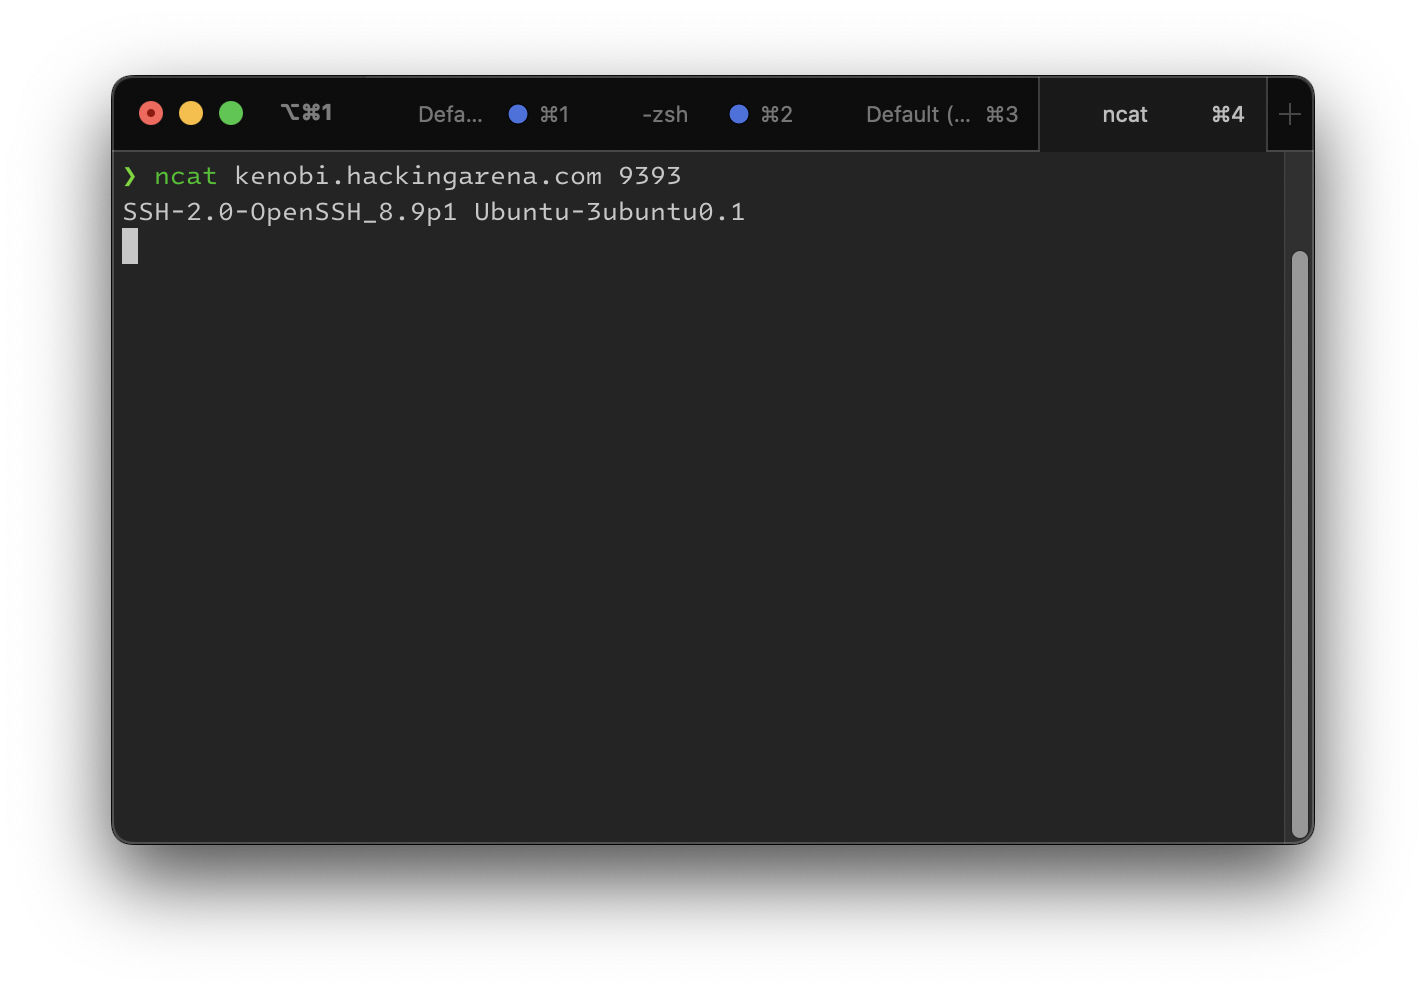
\includegraphics[width=15cm]{img/Get in touch with services/Casanova/Skjermbilde 2023-10-27 kl. 09.04.00.png}
\end{center}

That told me that an ssh service was running on the instance. I then figured the <<Ashley Madison case>> was a hint to a password breach, so i searched for it and found the top 100 passwords from the breach. I put the 100 passwords in a file called \texttt{passwrd.txt} and used hydra to brute force the password for the user \texttt{casanova} on the ssh service as such:

\begin{center}
    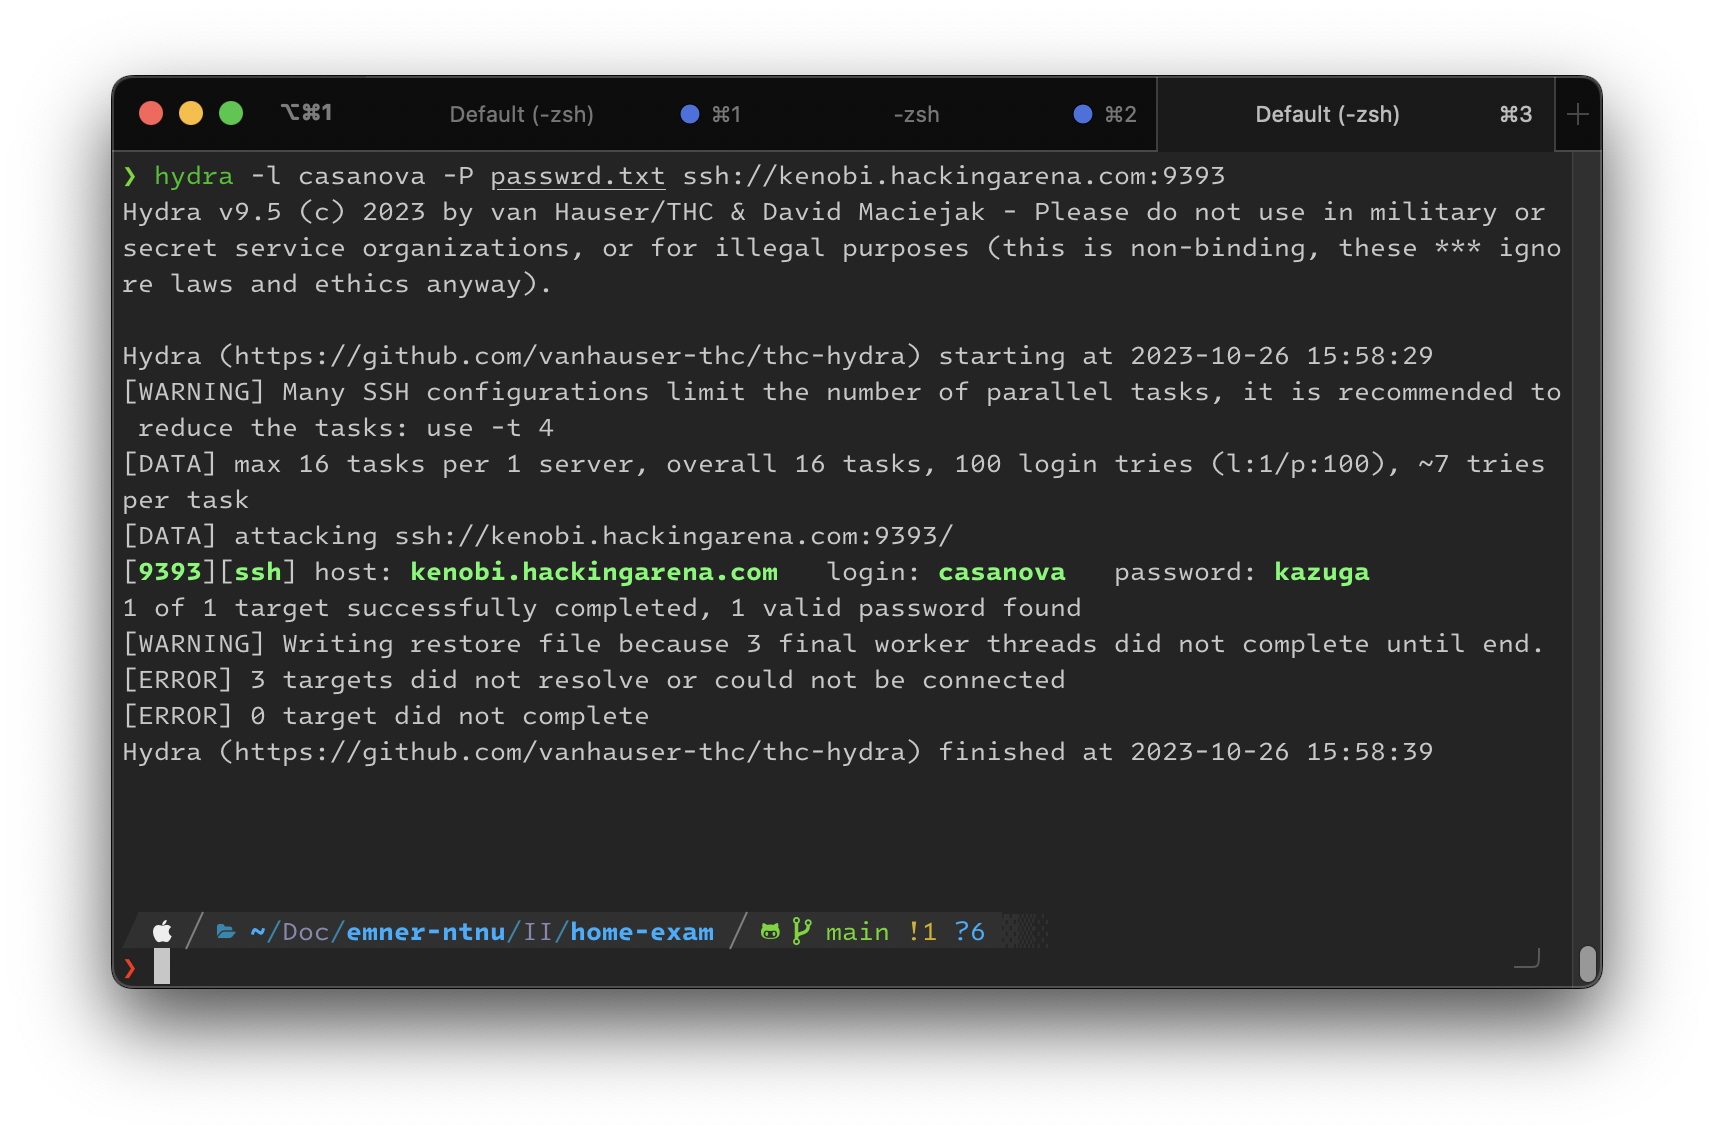
\includegraphics[width=15cm]{img/Get in touch with services/Casanova/Skjermbilde 2023-10-26 kl. 15.59.05.png}
\end{center}

I then got one hit, and the password was \texttt{kazuga}. I then connected to the service with ssh and found the flag in the home directory.

\begin{center}
    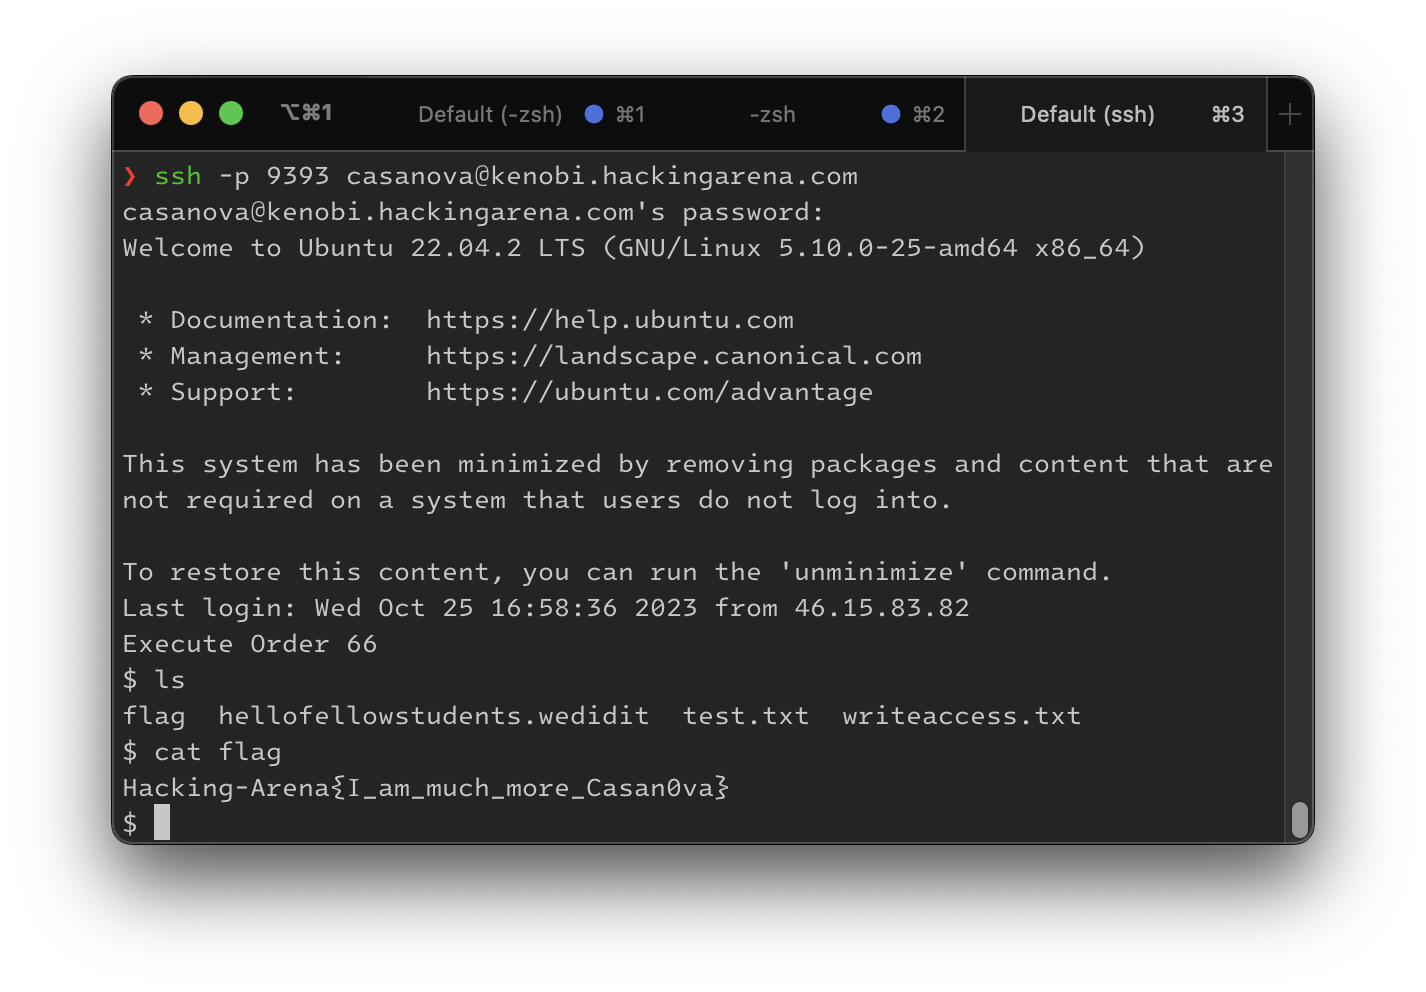
\includegraphics[width=15cm]{img/Get in touch with services/Casanova/Skjermbilde 2023-10-26 kl. 15.59.48.png}
\end{center}

The flag is: \texttt{Hacking-Arena\string{I\_am\_much\_more\_Casan0va\string}}

\newpage
\subsection{Minuteman (80p)}
A service is running on \texttt{kenobi.hackingarena.com} portrange: \texttt{7000-7500}. I hope you can find this very important flag :)

\textbf{Solution:}\\
I started by scanning the ports with nmap, and got the following output:

\begin{center}
    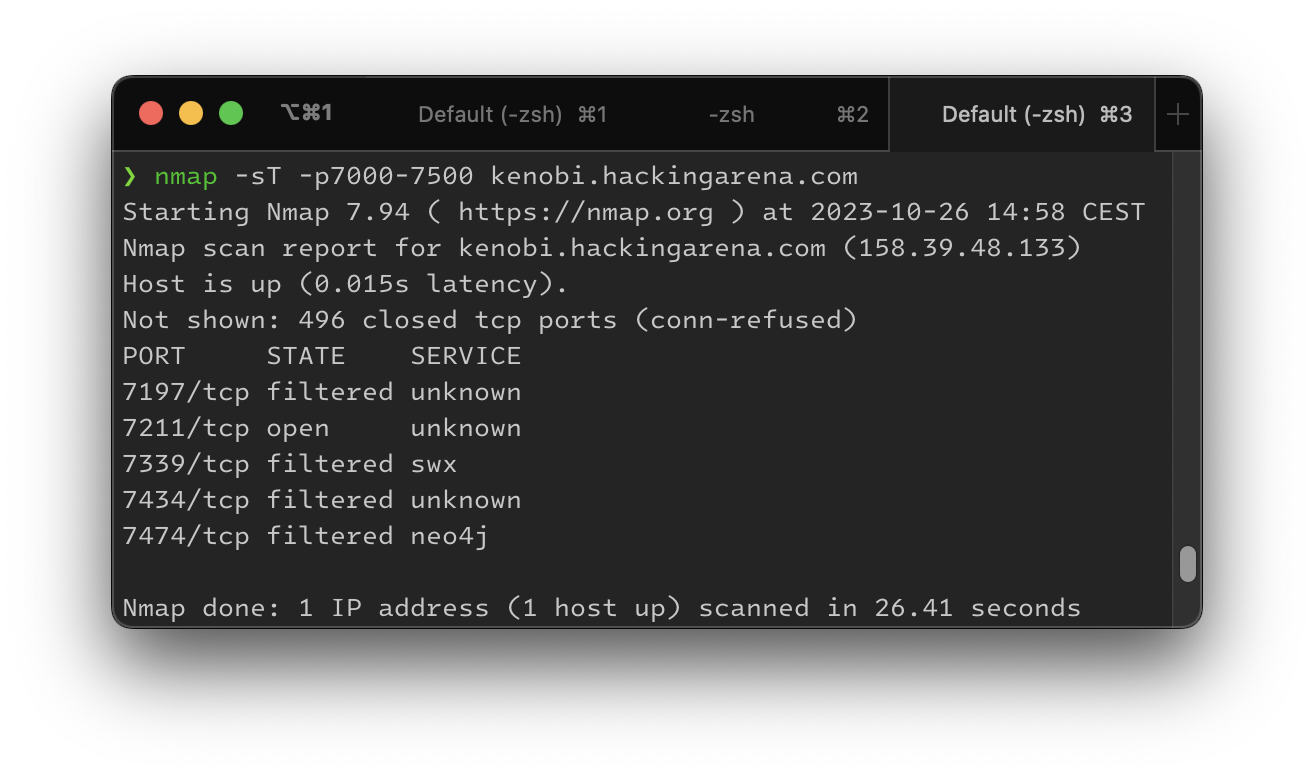
\includegraphics[width=14cm]{img/Get in touch with services/Minuteman/Skjermbilde 2023-10-26 kl. 15.14.45.png}
\end{center}

I then connected to the only open service on port 7211 with telnet, and got the following response:

\begin{center}
    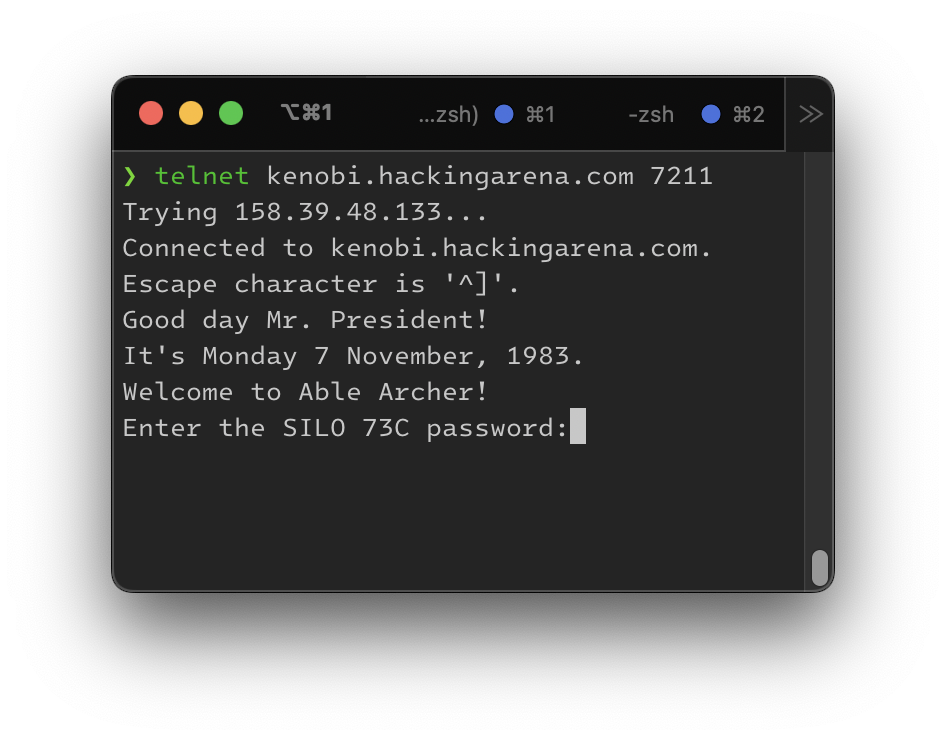
\includegraphics[width=11cm]{img/Get in touch with services/Minuteman/Skjermbilde 2023-10-27 kl. 09.30.39.png}
\end{center}

After searching for what Able Archer was, i found that it was a NATO exercise in 1983. I then found the nuclear launch codes for the exercise, which was \texttt{00000000}. I then connected to the service again with telnet, gave it the launch codes, and got the following response:

\begin{center}
    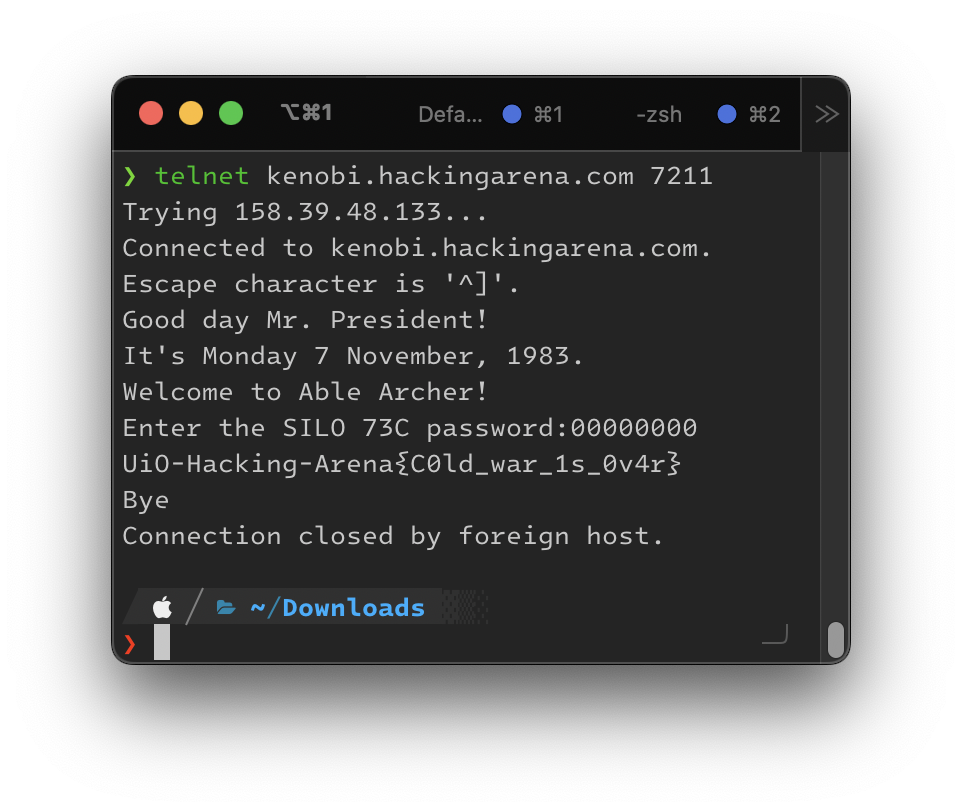
\includegraphics[width=12cm]{img/Get in touch with services/Minuteman/Skjermbilde 2023-10-26 kl. 15.13.55.png}
\end{center}

The flag was \texttt{UiO-Hacking-Arena\string{C0ld\_war\_1s\_0v4r\string}}.

\newpage
\subsection{Dark energy (90p)}
Have you already checked padawan ports? What was this on \texttt{tcp/502}? Maybe there is a flag for you. :)

\textbf{Solution:}\\
First i had to check again what service was running on port 502, and found that it was modbus.
I then downloaded a \href{https://github.com/tallakt/modbus-cli}{modbus client} and followed the README instructions and ran the command:
\texttt{modbus read -p502 padawan.hackingarena.com \%MW100 50}
which read 50 registers from the modbus server on port 502.

\begin{center}
    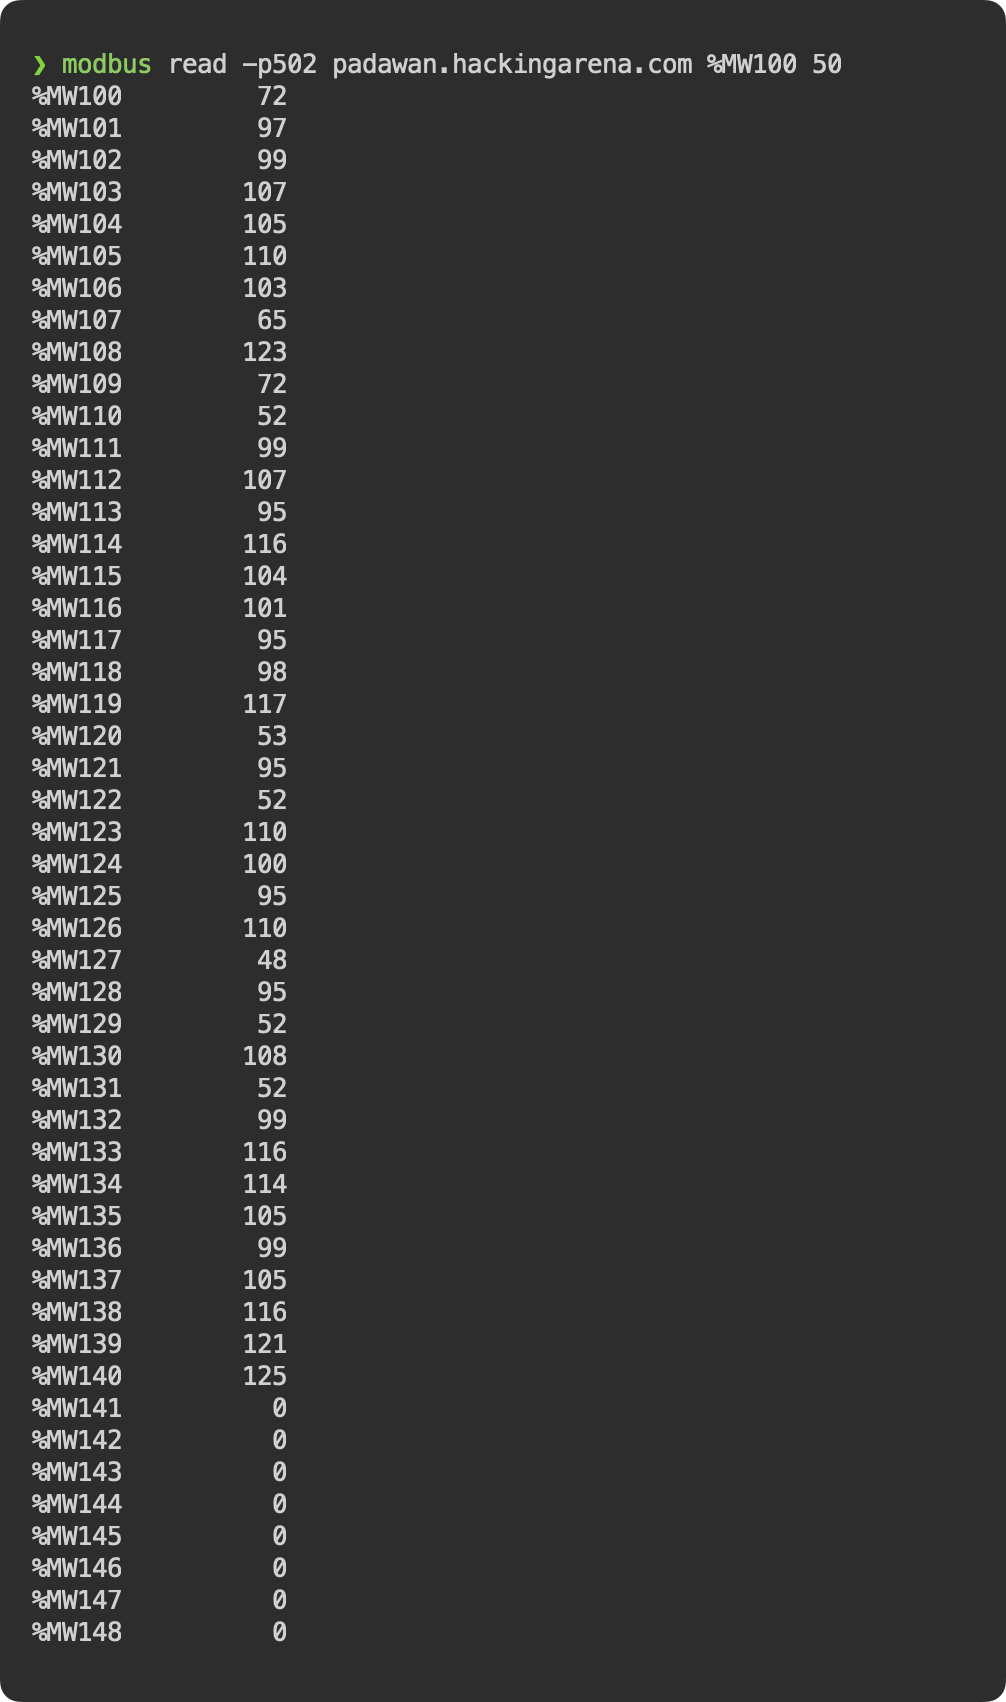
\includegraphics[width=9cm]{img/Get in touch with services/Dark energy/Screenshot 2023-11-10 at 10.38.21.png}
\end{center}

I then copied the numbers from the output and converted them from decimal to ascii, and got the following flag:
\texttt{HackingA\string{H4ck\_the\_bu5\_4nd\_n0\_4l4ctricity\string}}
\section{Web Hacking}

\subsection{Beatles song catalogue (60p)}
There must be something hidden here:
\url{http://r2d2.hackingarena.com:1811}

\textbf{Solution:}\\
I first connected to the site with Burp Suite and explored the different sites. The parameter for switching sites was \texttt{songid}, and after finding the pattern with the albums that all ended with \texttt{53} i set up an intruder attack with the following payload:

\begin{center}
    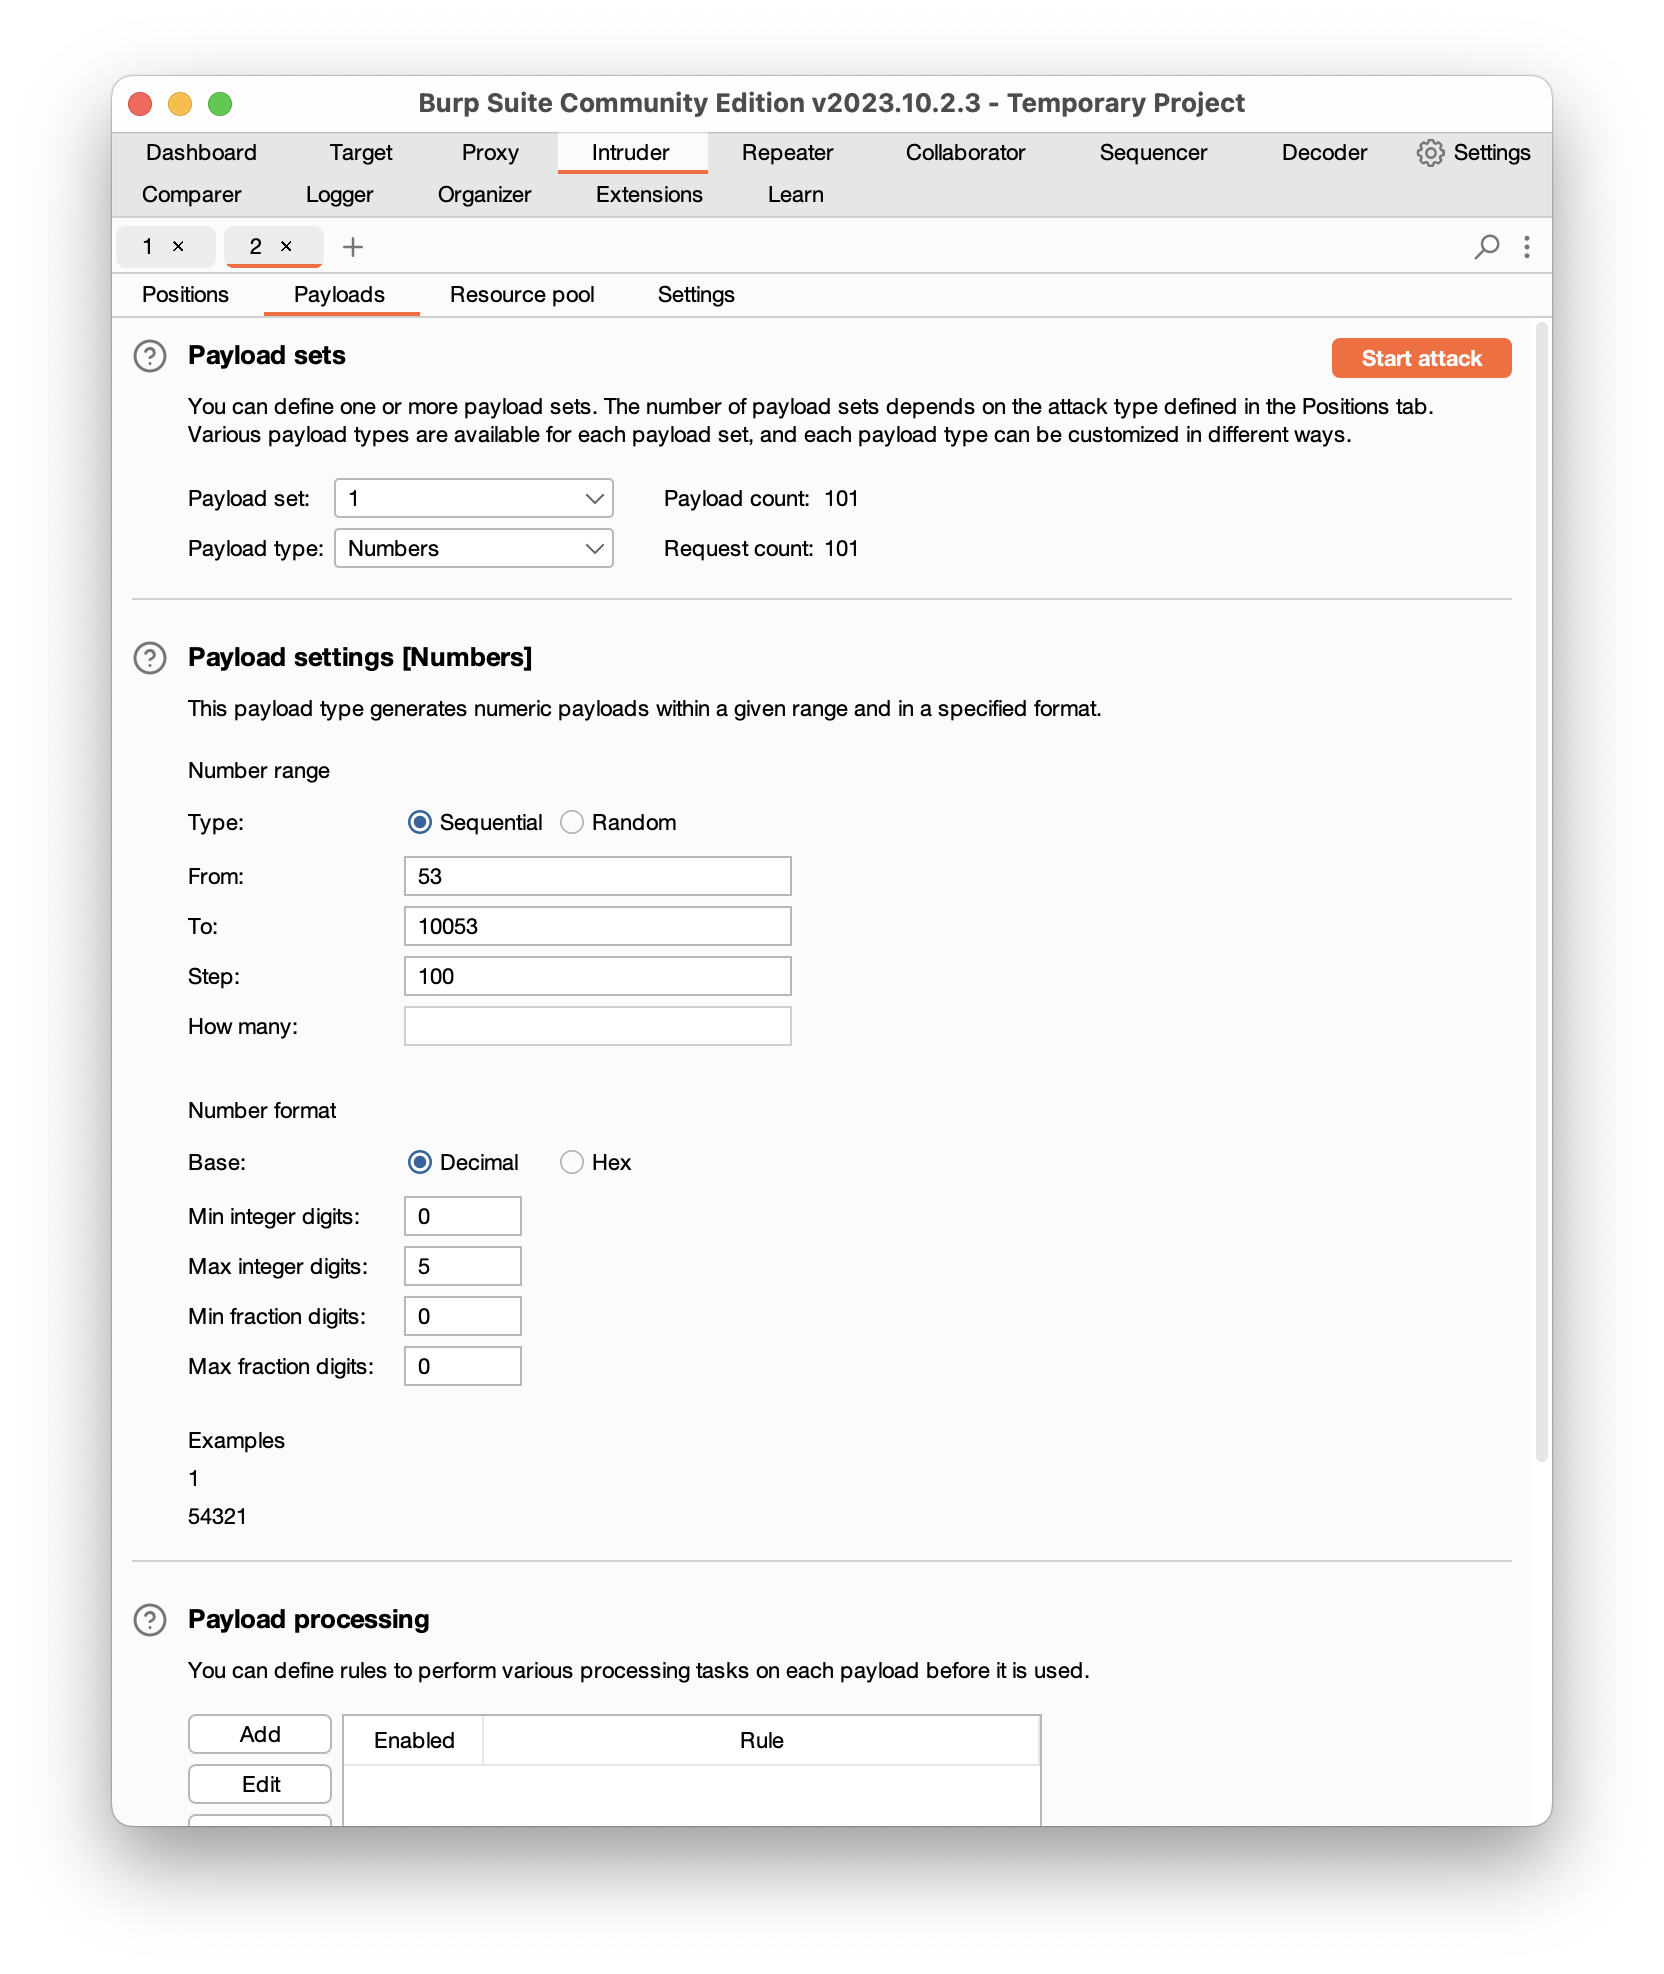
\includegraphics[width=15cm]{img/Web hacking/Beatles song catalogue/Skjermbilde 2023-10-26 kl. 13.06.47.png}
\end{center}

When the attack was done I searched through the results that had a length other than 232 or 233 since these were empty pages. I found the following page:

\begin{center}
    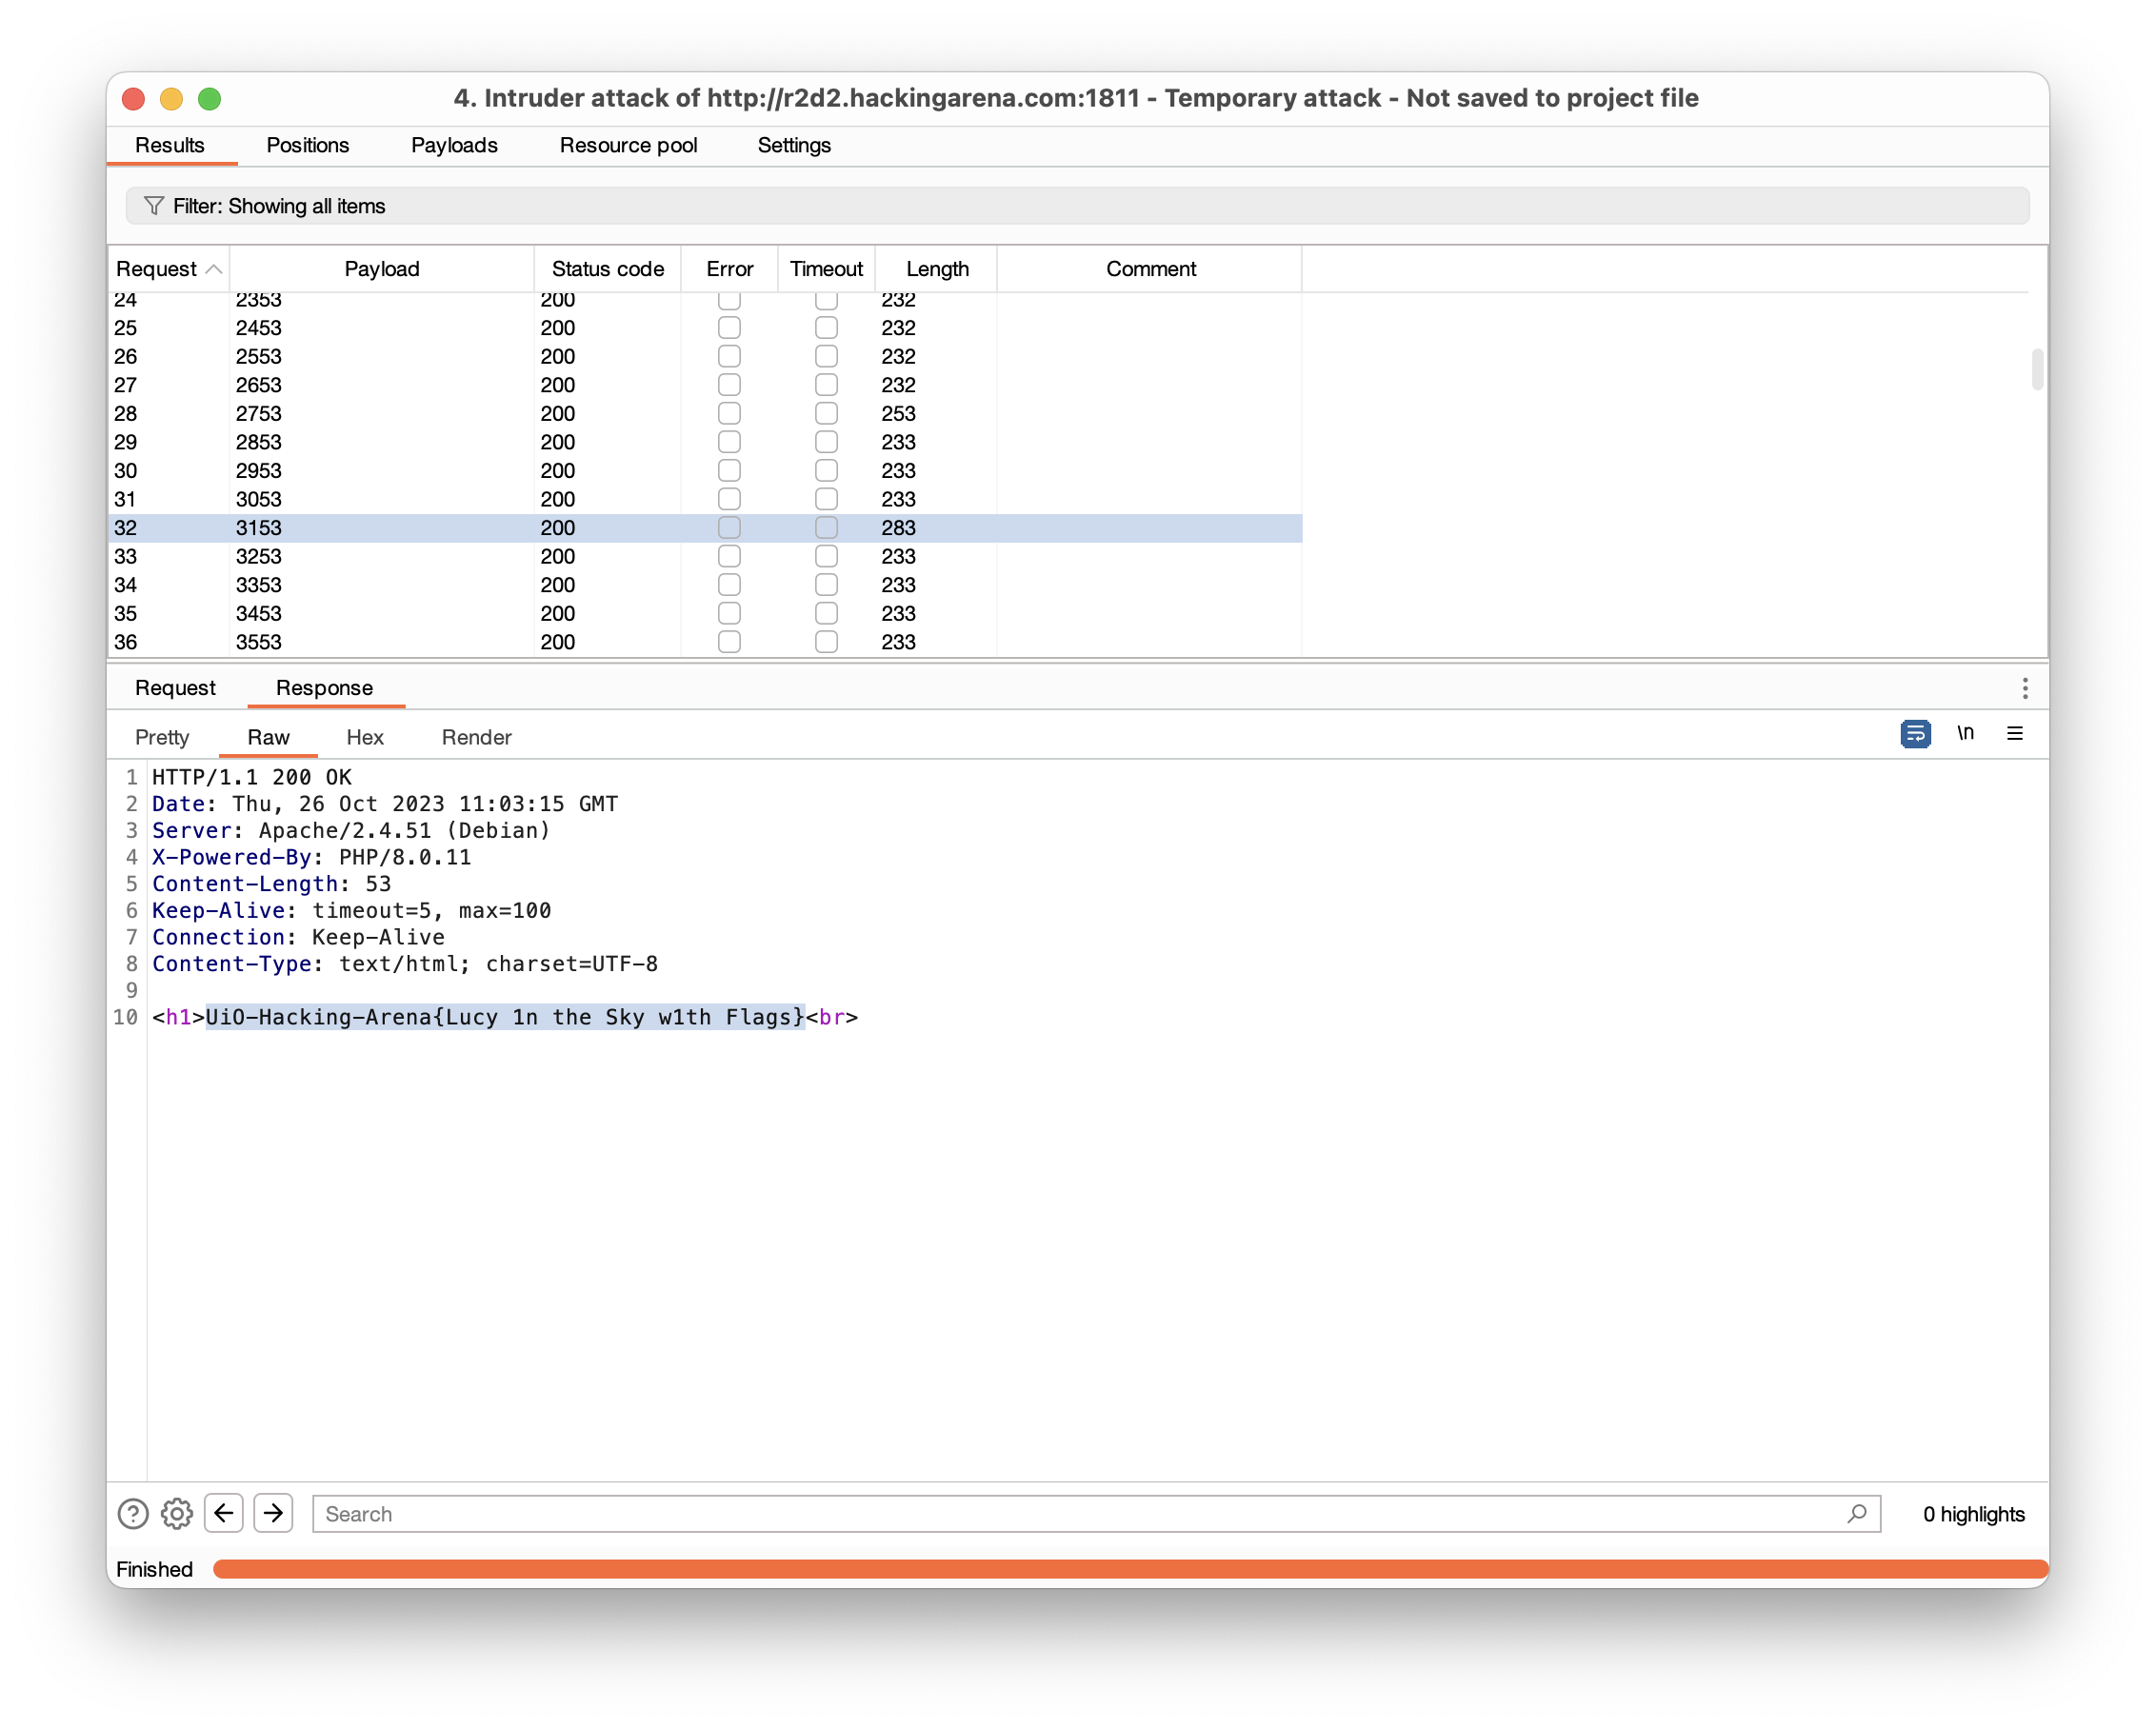
\includegraphics[width=15cm]{img/Web hacking/Beatles song catalogue/Skjermbilde 2023-10-26 kl. 13.06.58.png}
\end{center}

The flag is: \texttt{UiO-Hacking-Arena\string{Lucy 1n the Sky w1th Flags\string}}

\newpage
\subsection{Web 5 (60p)}
Can you find the flag here?
\url{http://padawan.hackingarena.com:820}

\textbf{Solution:}\\
The trick I found to solving this task was exceeding the character limit of the input field. When I did this I got the following error message:

\begin{center}
    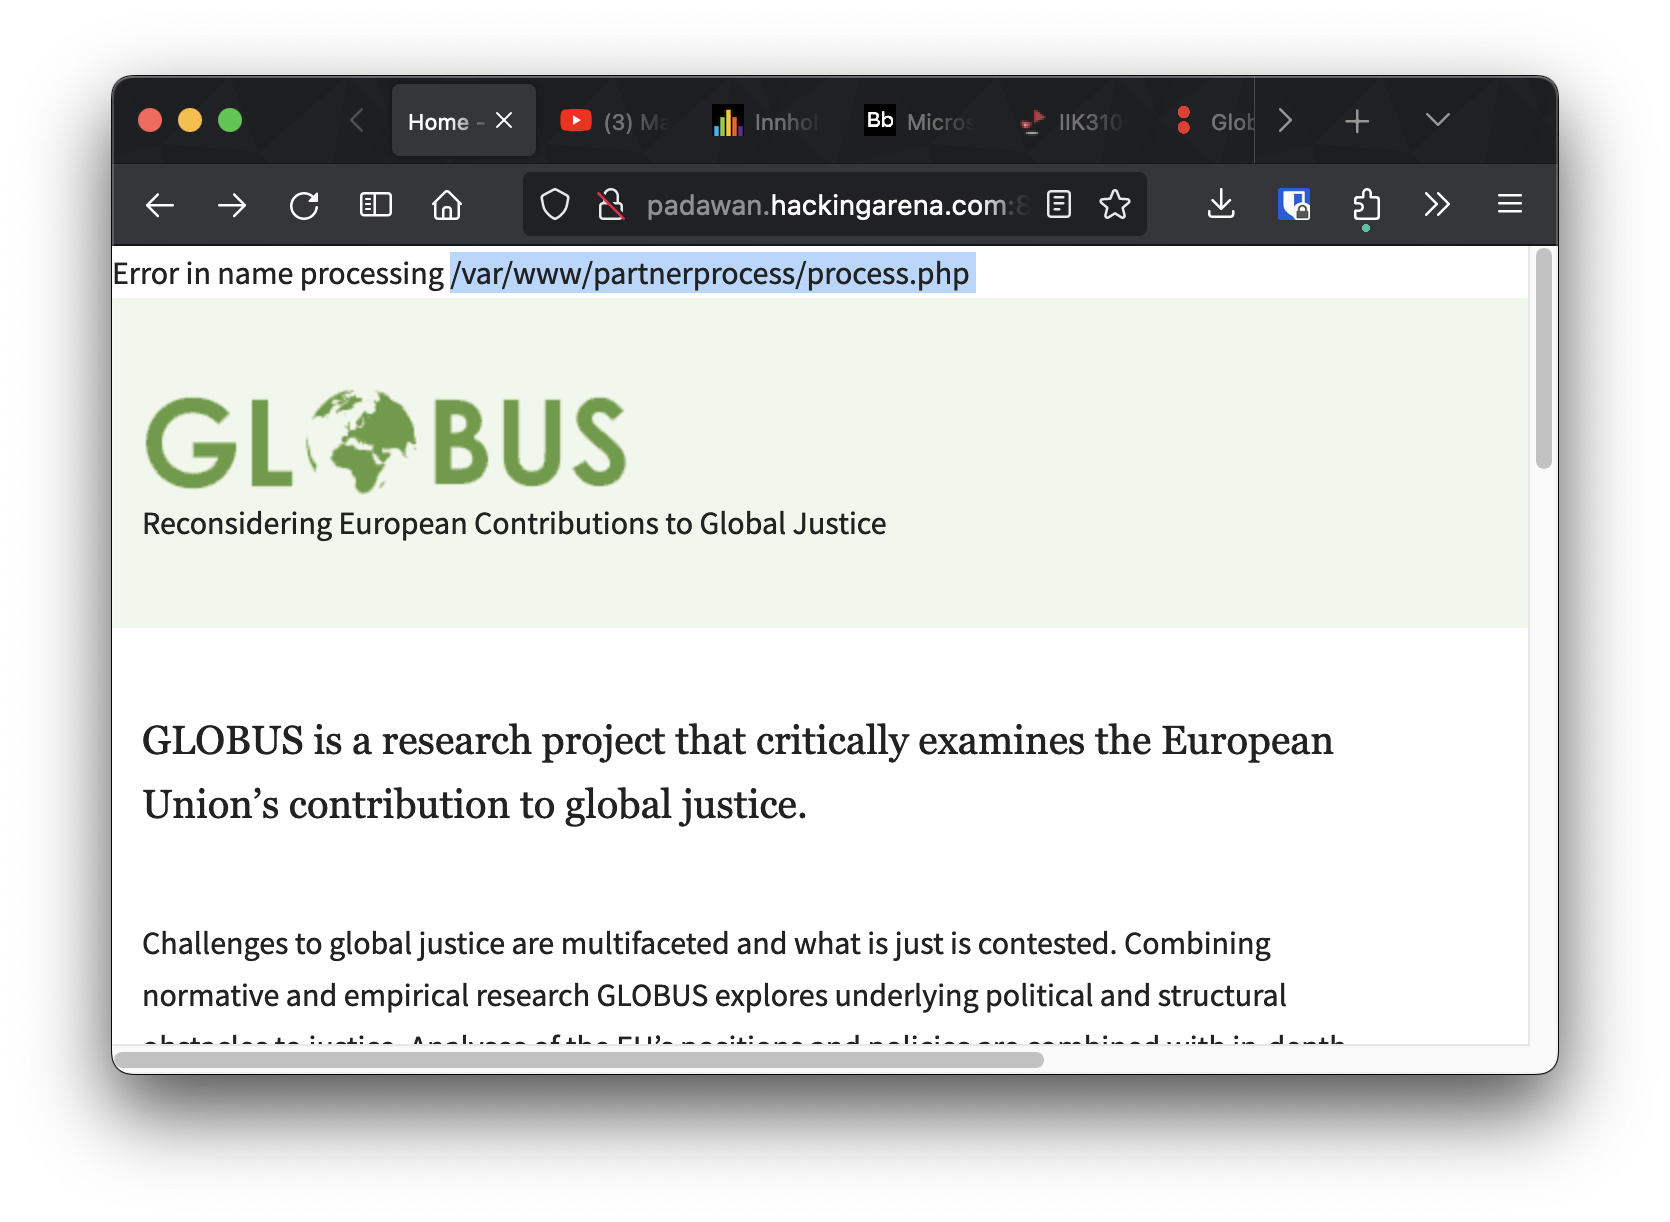
\includegraphics[width=12cm]{img/Web hacking/Web 5/Skjermbilde 2023-10-26 kl. 13.37.52.png}
\end{center}

Assuming the site was located at \texttt{/var/www/} I followed the path \texttt{partnerprocess/process.php}

\begin{center}
    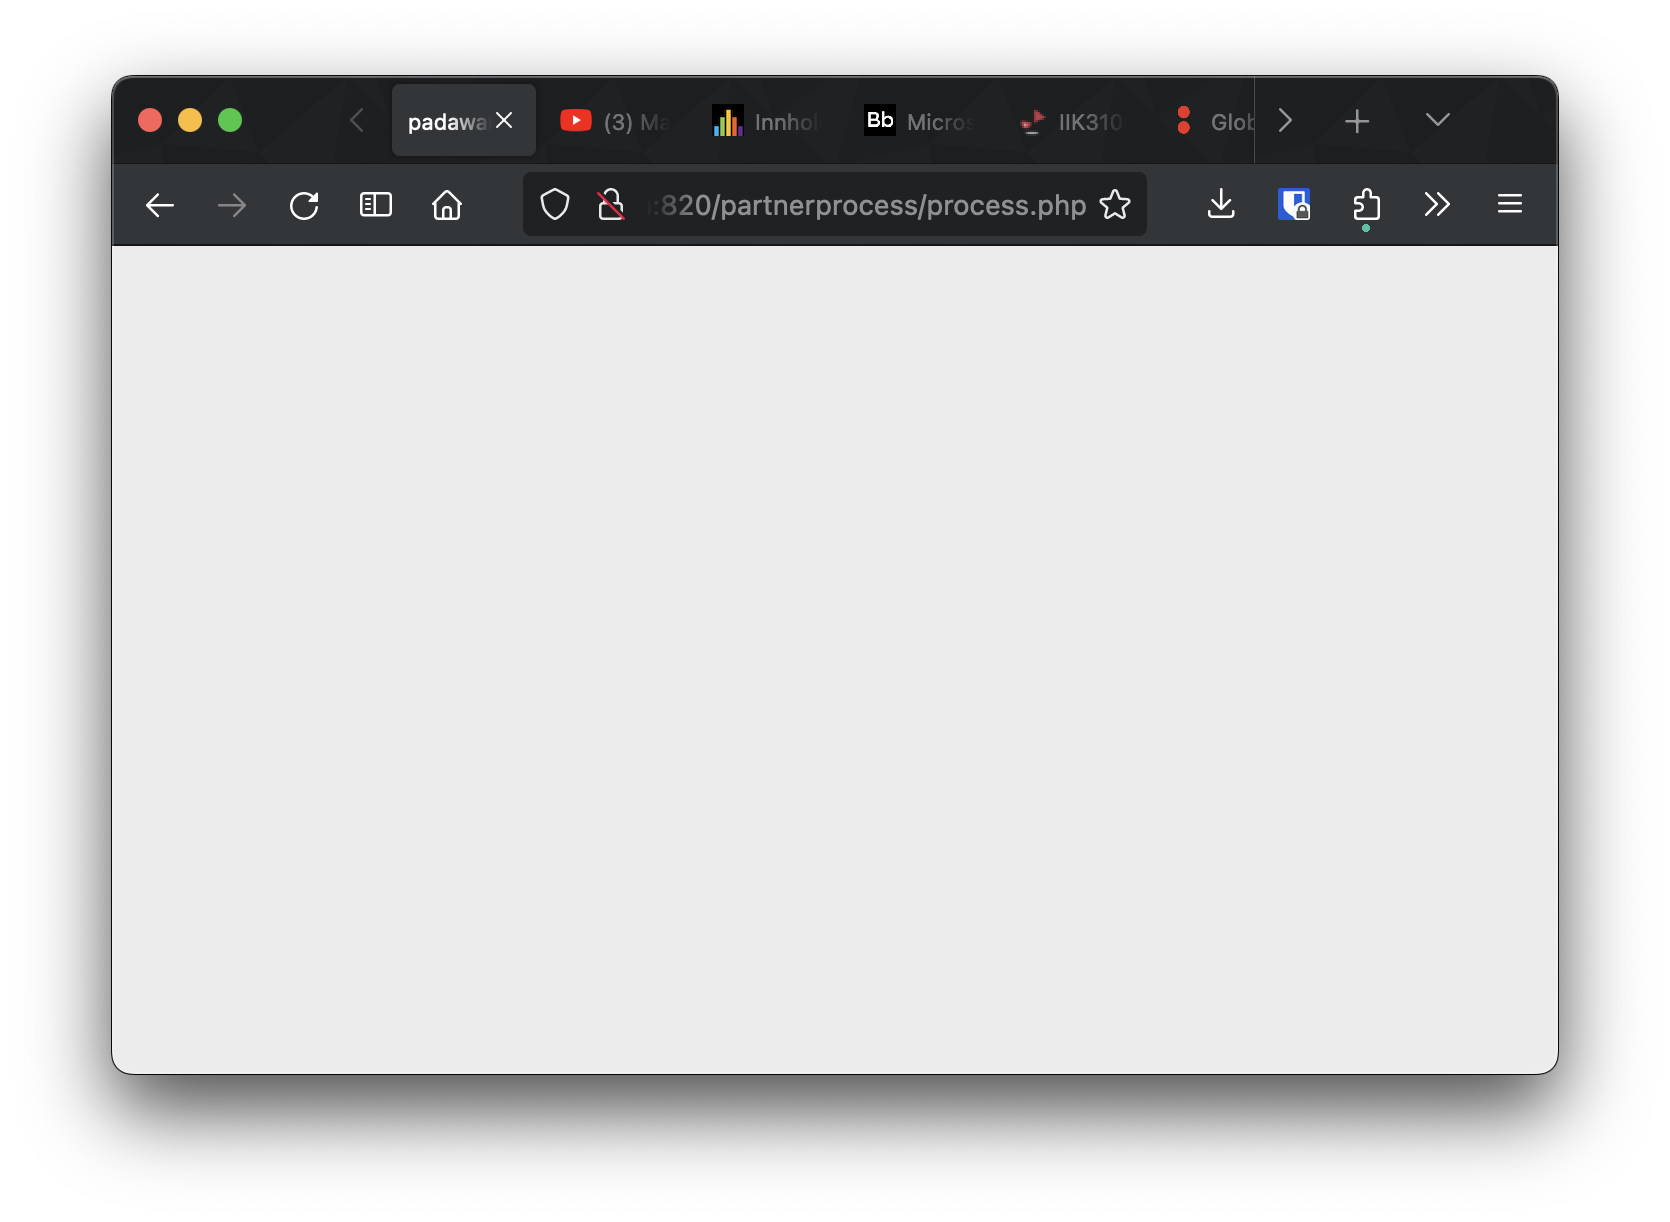
\includegraphics[width=12cm]{img/Web hacking/Web 5/Skjermbilde 2023-10-26 kl. 13.38.18.png}
\end{center}

After that I jumped to the parent directory \texttt{partnerprocess/} and found the flag in the \texttt{flag.txt} file.

\begin{center}
    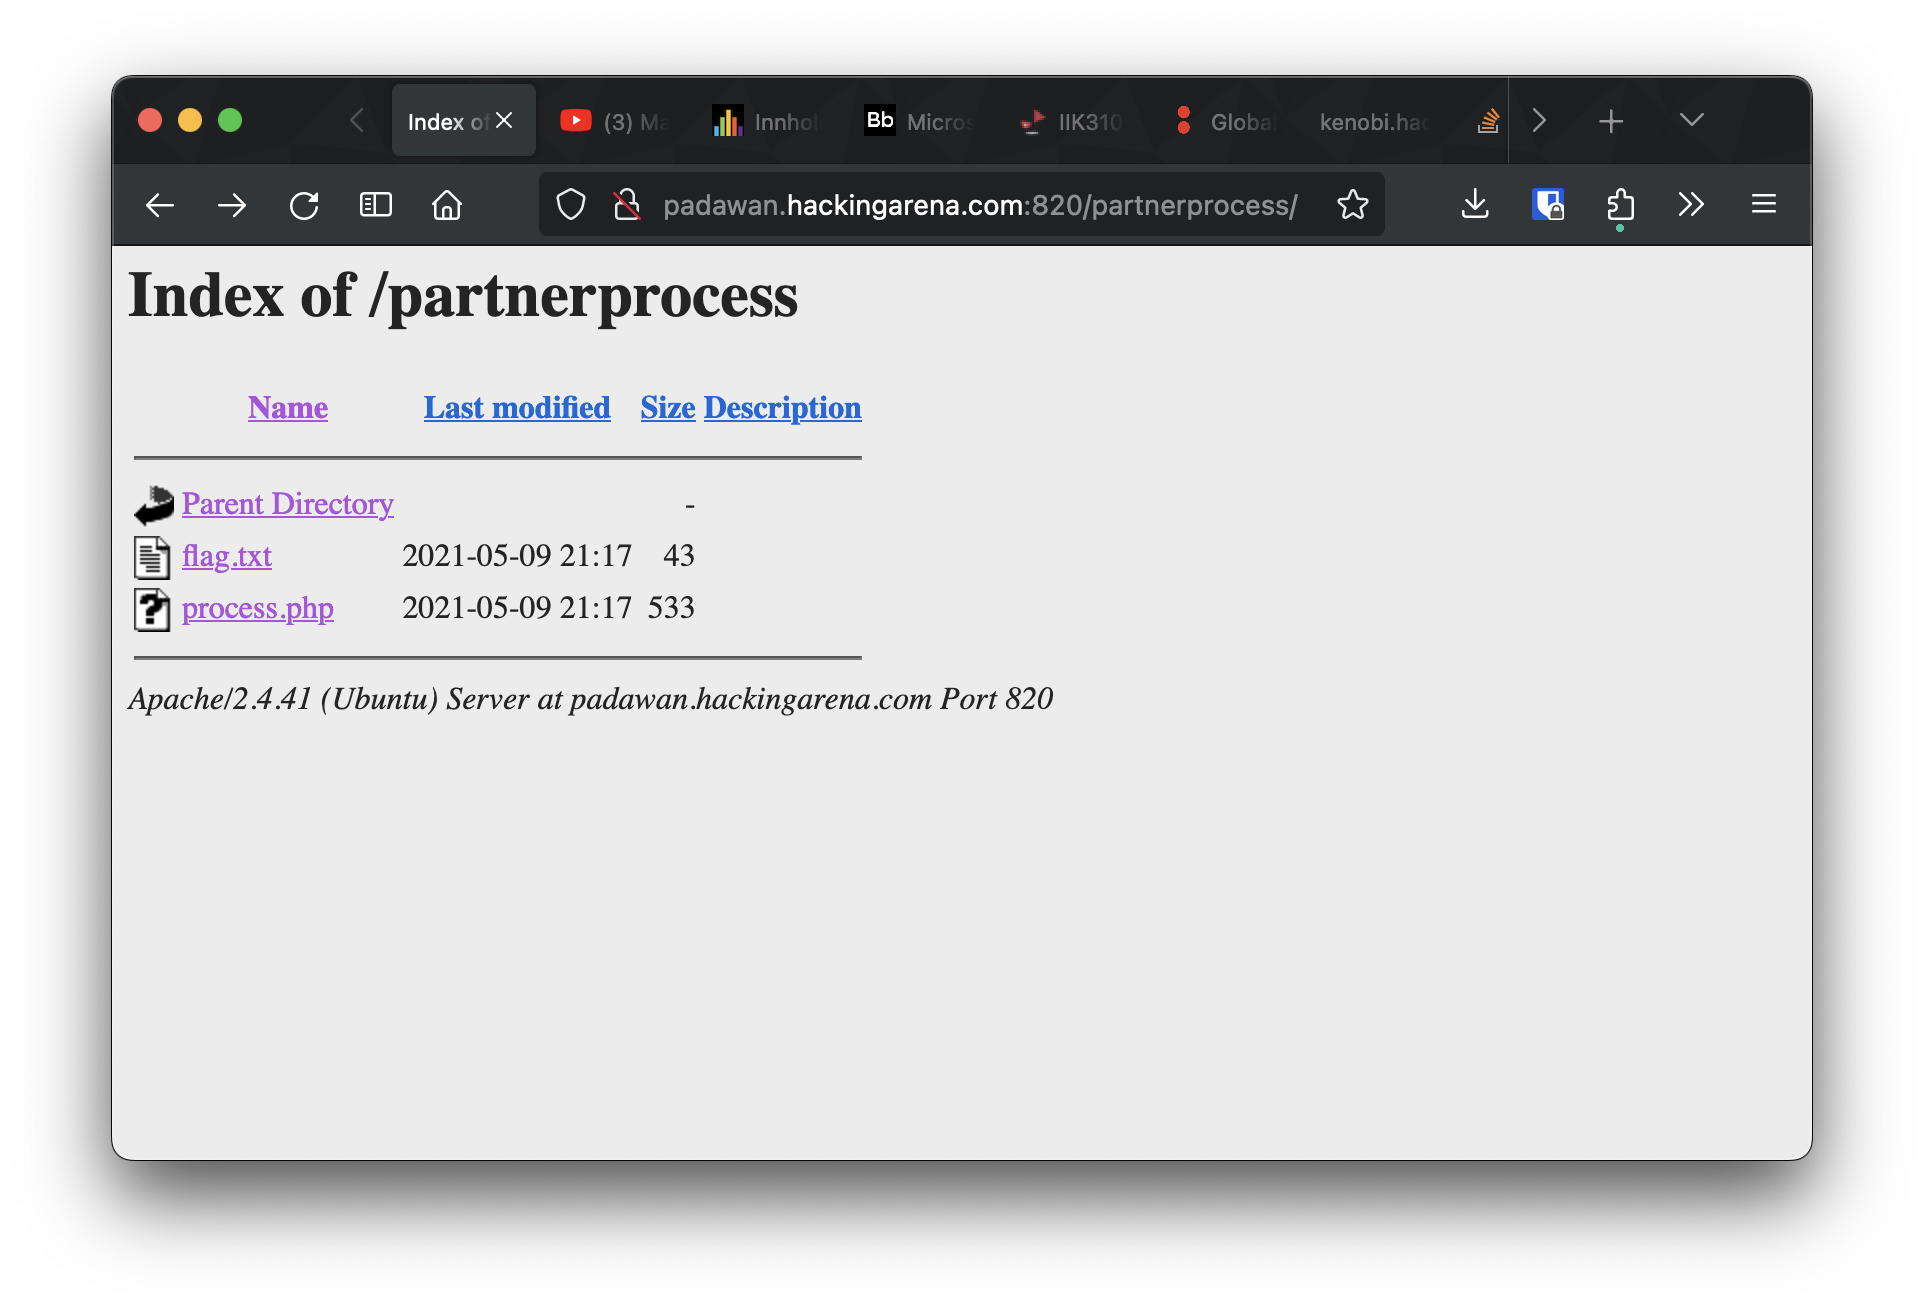
\includegraphics[width=12cm]{img/Web hacking/Web 5/Skjermbilde 2023-10-26 kl. 13.37.19.png}
\end{center}

Opening the file revealed the flag:

\begin{center}
    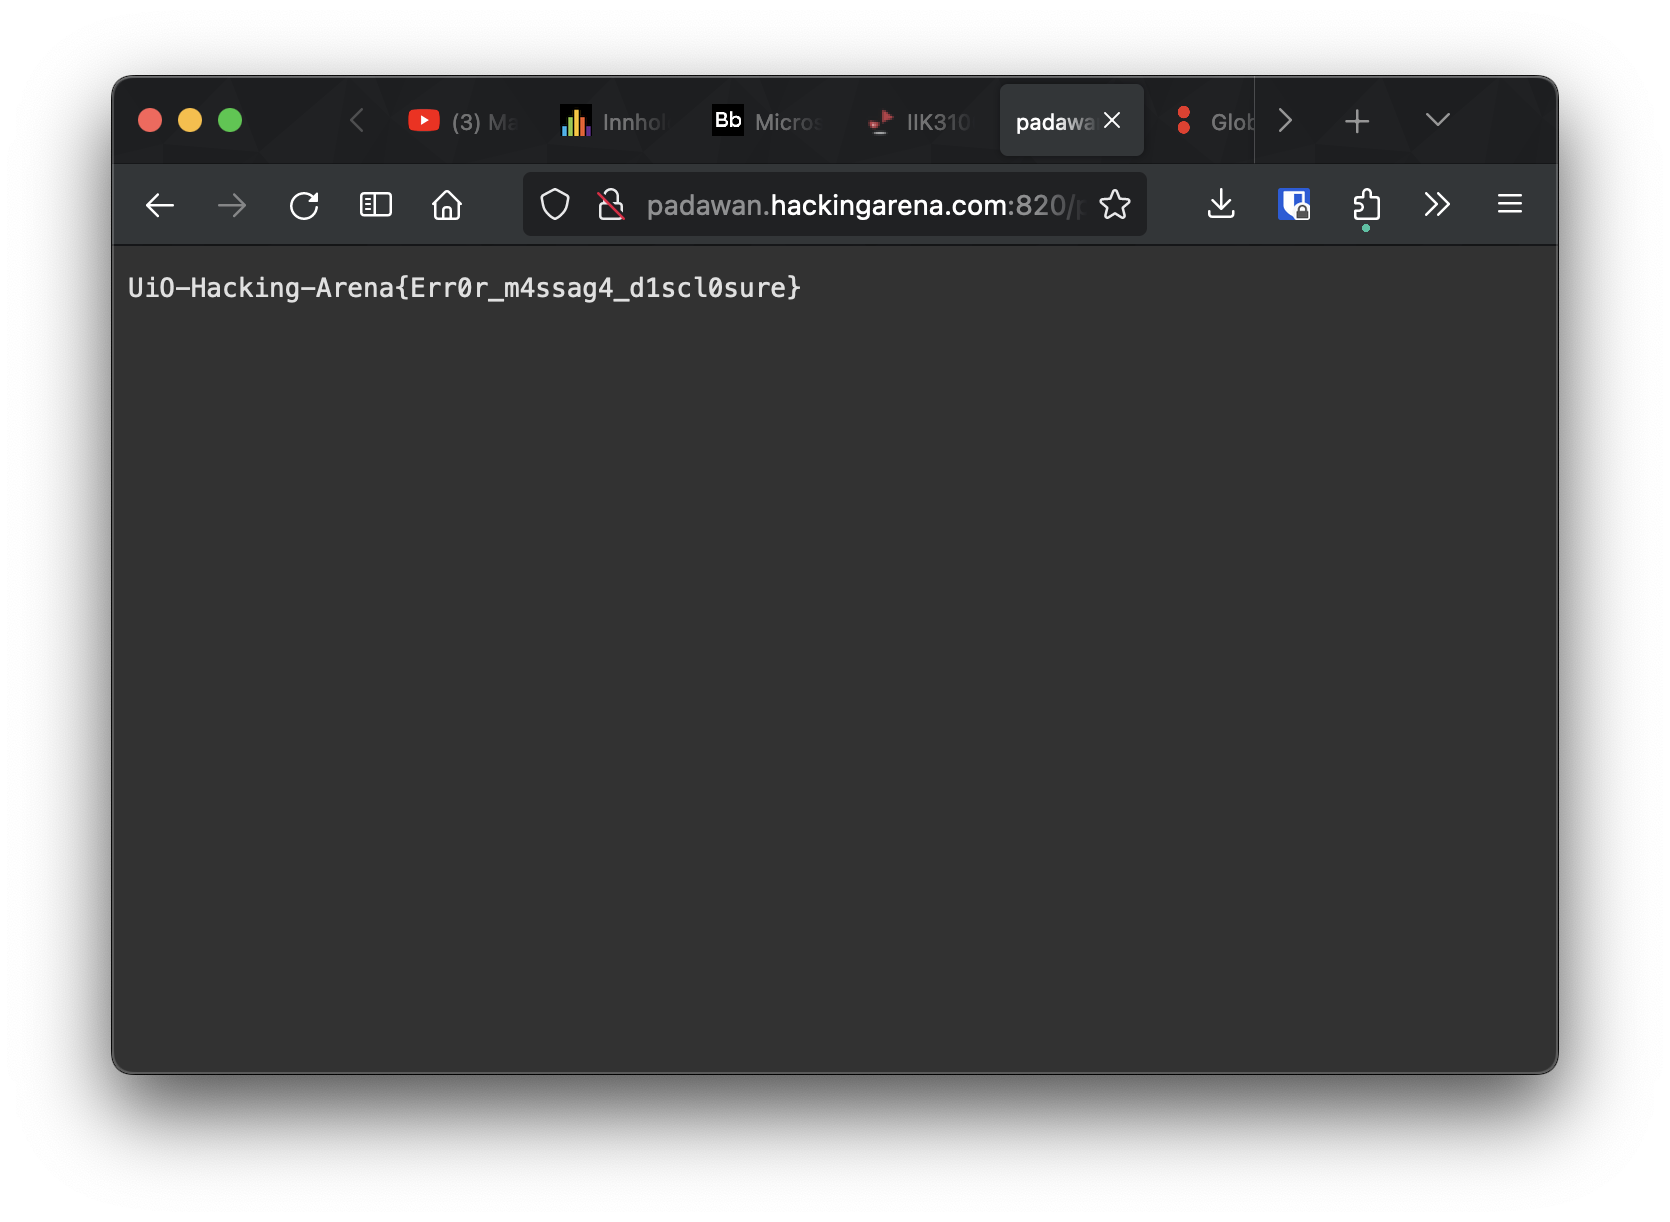
\includegraphics[width=12cm]{img/Web hacking/Web 5/Skjermbilde 2023-10-26 kl. 13.39.25.png}
\end{center}

The flag is: \texttt{UiO-Hacking-Arena\string{Err0r\_m4ssag4\_d1scl0sure\string}}

\newpage
\subsection{Redirect (60p)}
Can you redirect \texttt{kenobi.hackingarena.com:821} to \texttt{kenobi.hackingarena.com:822}?

\textbf{Solution:}\\
This task was all about cross site scripting. I first tried to inject a script into the input field, but this did not work. 
I then tried to log to the console with the injected script, but I realized some anti tampering mechanism was in place as I got a lot of \texttt{***ANTIHACKER***} in my log. 
I then had the idea of replacing the \texttt{window.location} with the new url.
This didn't work when injecting the script, so I tried again but this time in the console and it worked.

\begin{figure}[H]
    \centering
    \begin{minipage}{.5\textwidth}
        \hspace*{-1cm}
        \centerline{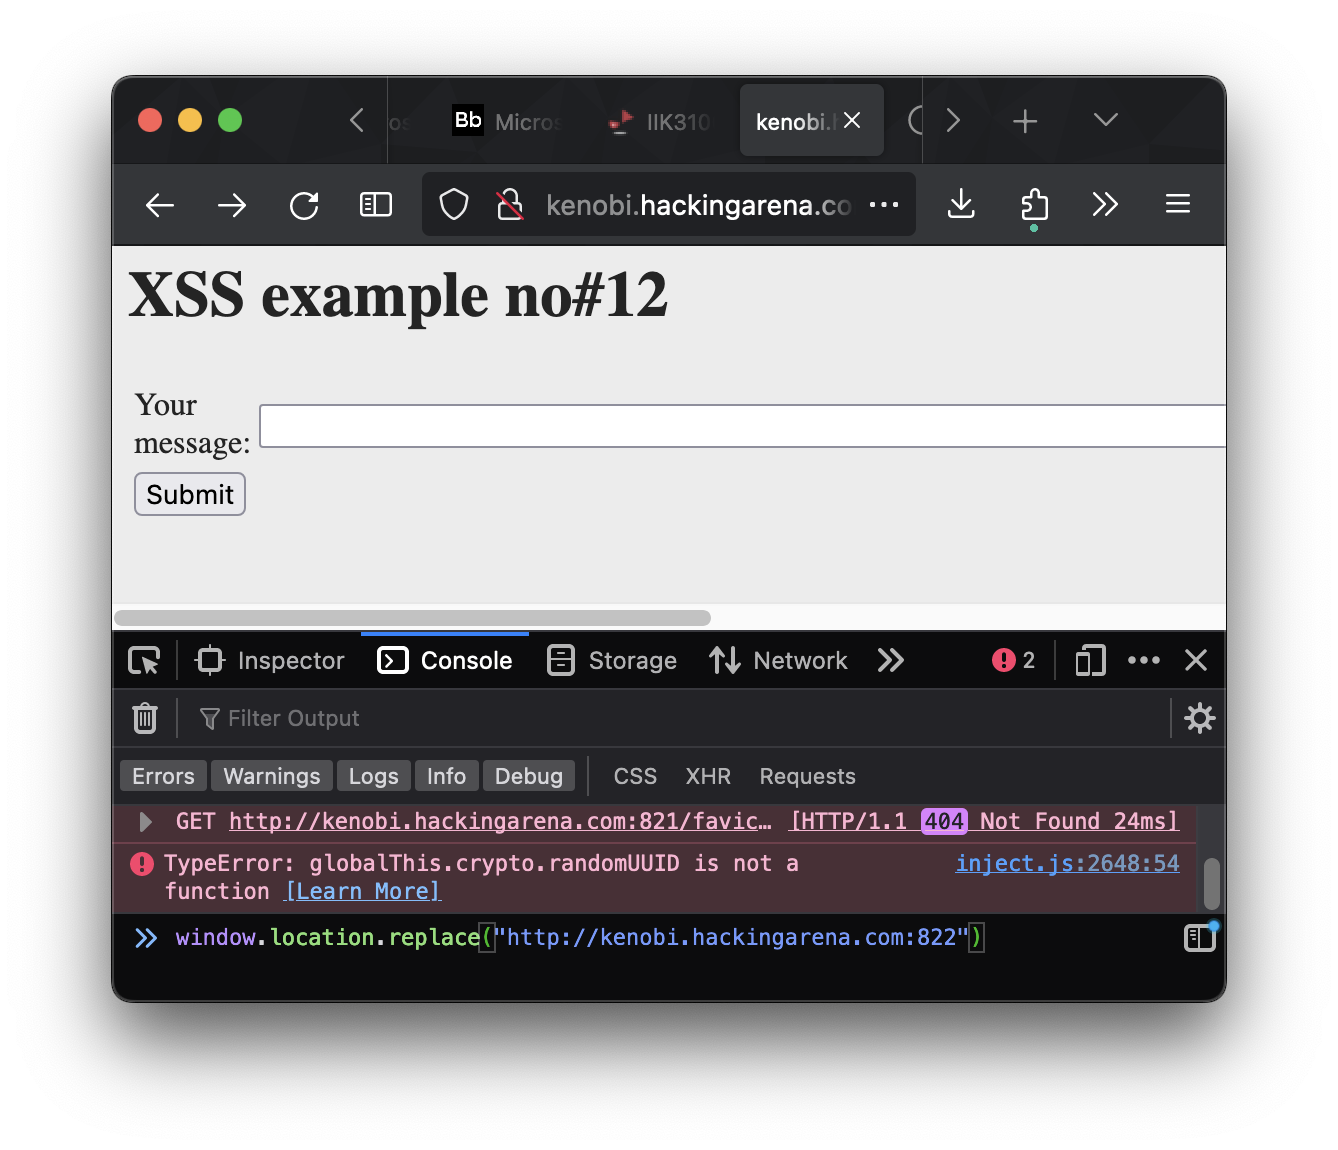
\includegraphics[width=1.4\textwidth]{img/Web hacking/Redirect/Skjermbilde 2023-10-26 kl. 15.29.27.png}}
        \vspace*{-.5cm}
        \captionof*{figure}{Before running the \\command in the console}
    \end{minipage}%
    \begin{minipage}{.5\textwidth}
        \hspace*{1cm}
        \centerline{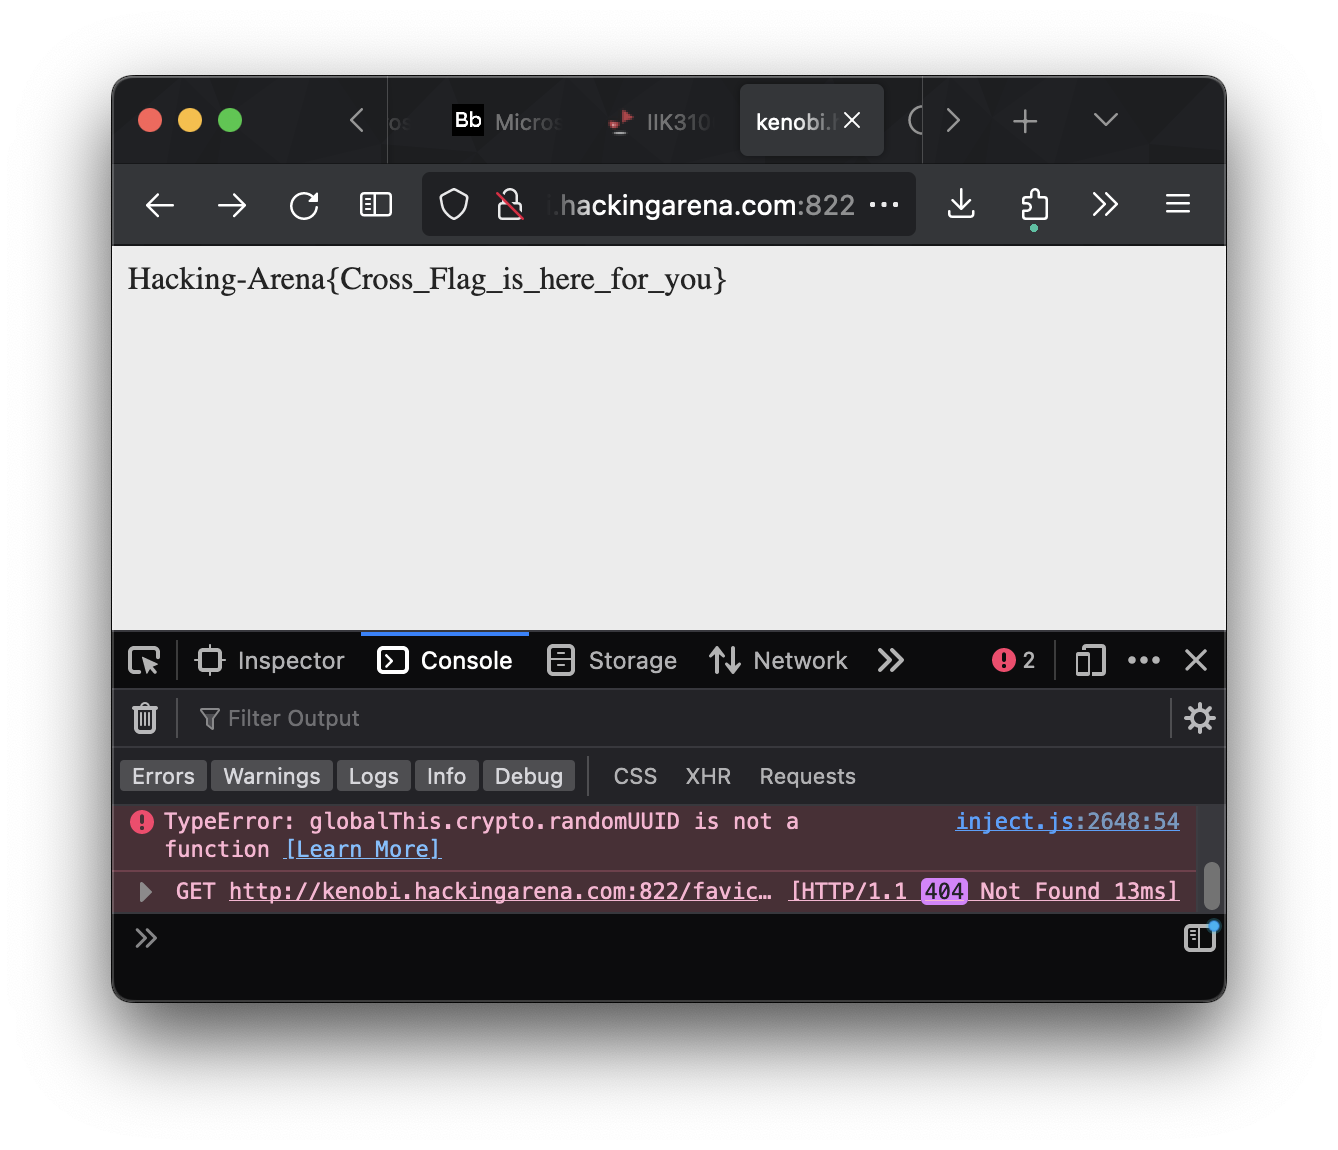
\includegraphics[width=1.4\textwidth]{img/Web hacking/Redirect/Skjermbilde 2023-10-26 kl. 15.29.41.png}}
        \vspace*{-1 cm}
        \captionof*{figure}{After running the \\command in the console}
    \end{minipage}
\end{figure}

\newpage
\subsection{Arenabook (80p)}
Hi, Check out the latest social media platform:
\url{http://sidious.hackingarena.com:803}
Sandra already tried it. :)

\textbf{Solution:}\\
The first step was to look for Sandra.

\begin{center}
    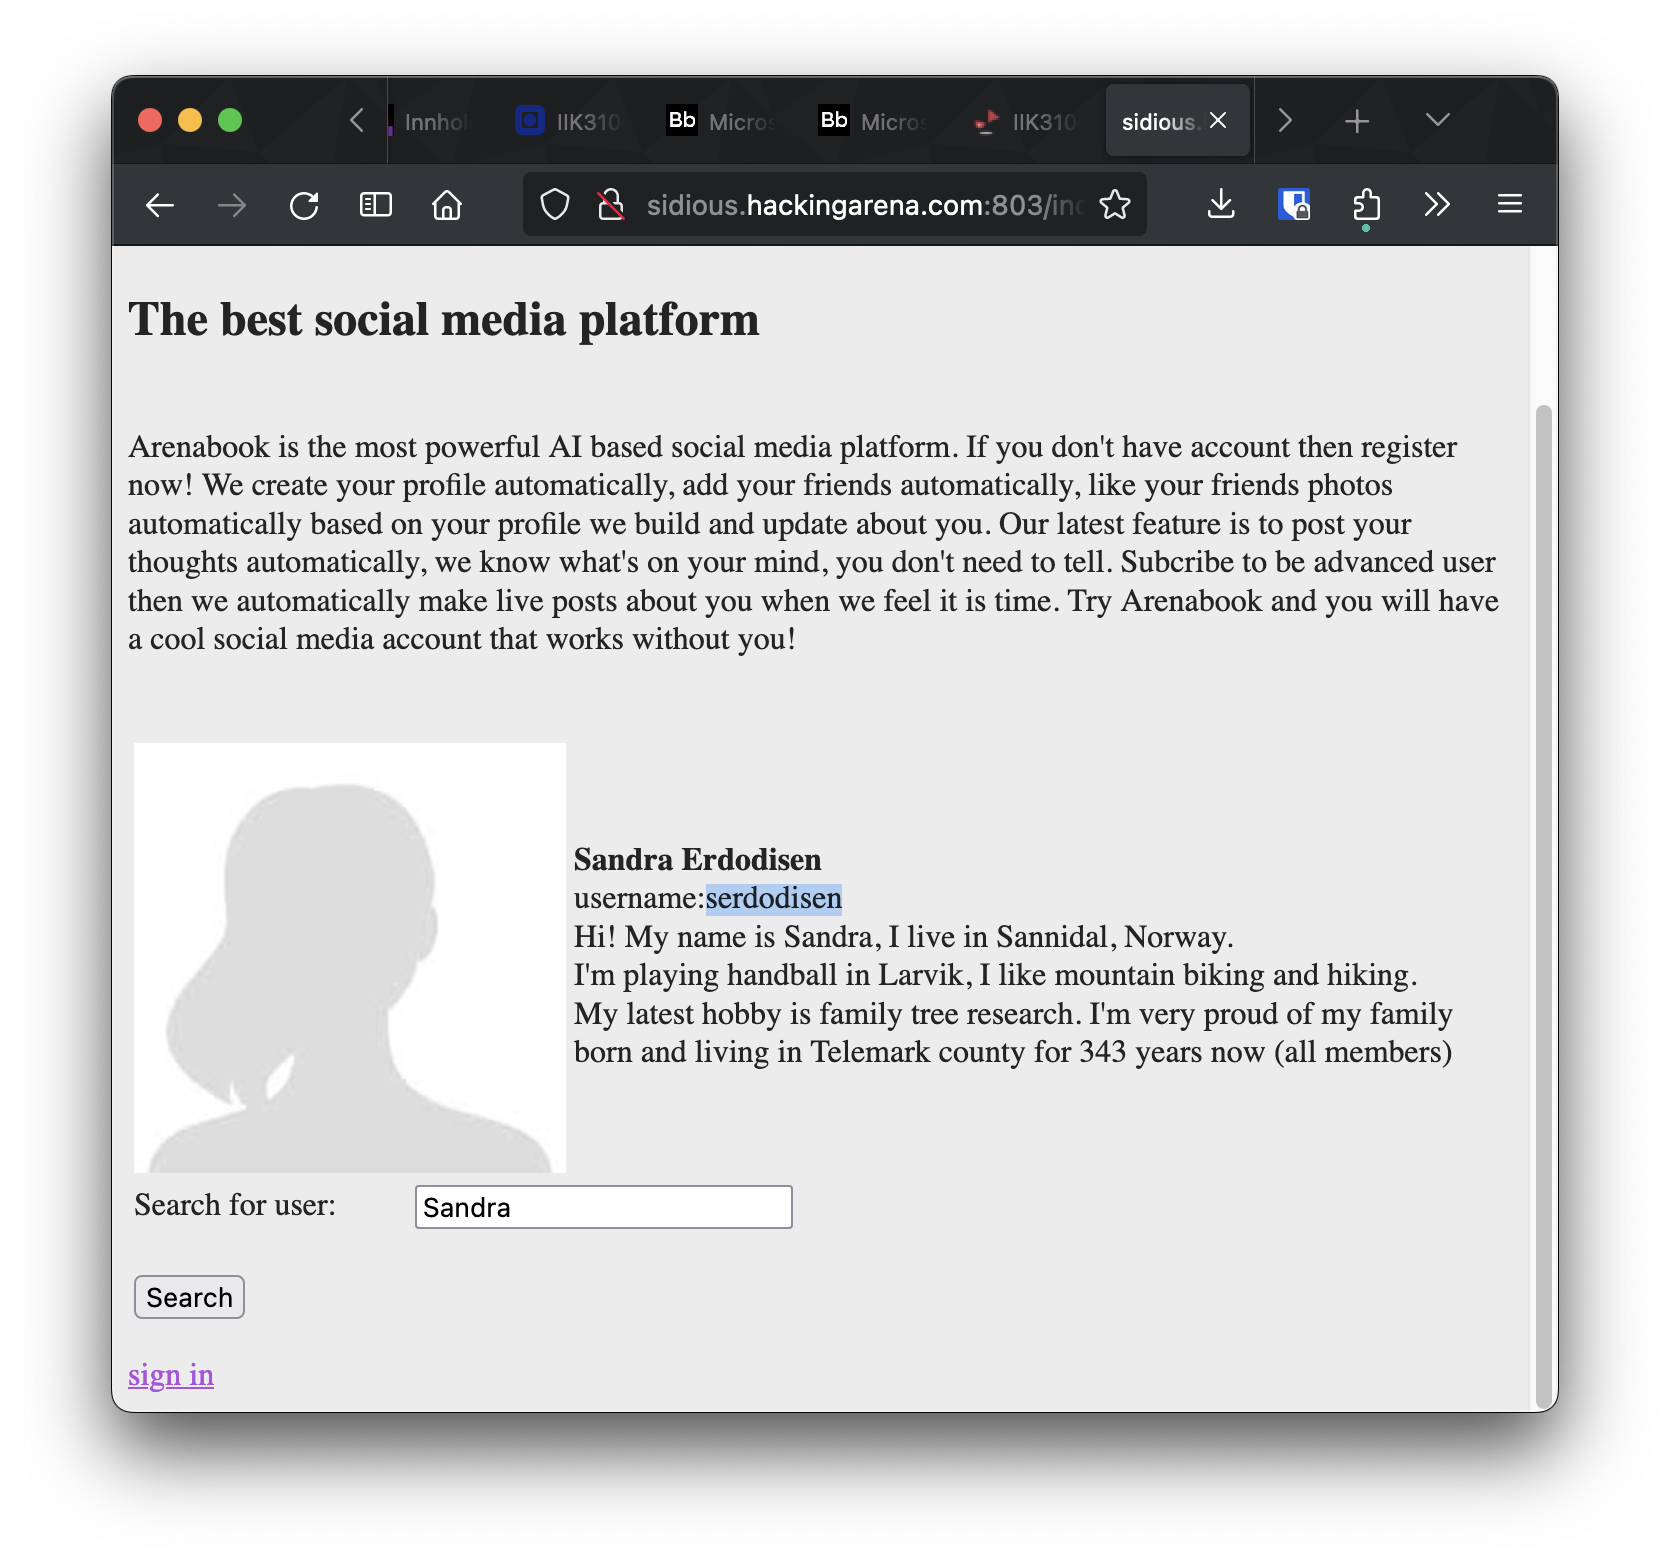
\includegraphics[width=12cm]{img/Web hacking/Arenabook/Skjermbilde 2023-10-26 kl. 14.49.43.png}
\end{center}

After getting her username I could use the forgot password function to get her password. I ended up at a page asking for the birthplace of her grandmother.

\begin{center}
    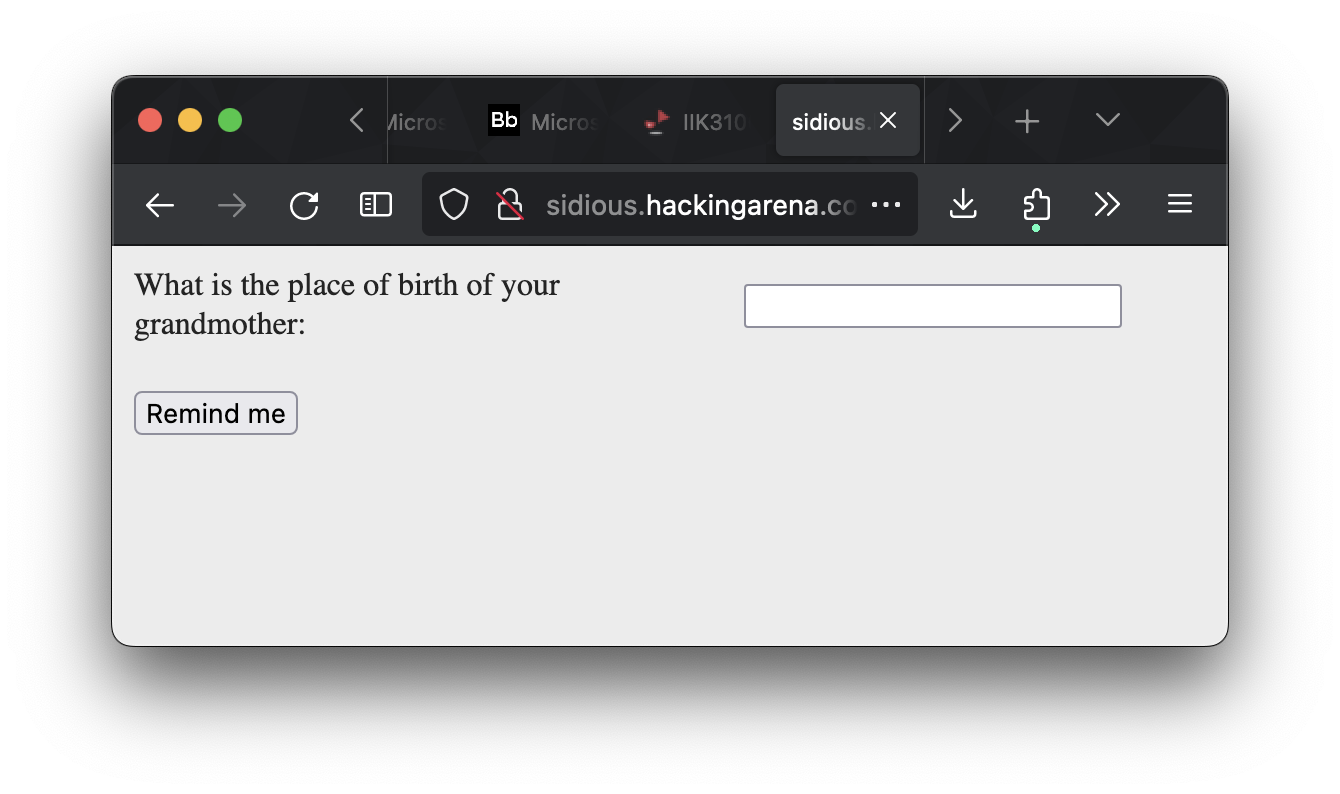
\includegraphics[width=12cm]{img/Web hacking/Arenabook/Skjermbilde 2023-10-26 kl. 14.50.02.png}
\end{center}

After putting this page into Burp Suite I found a field in the post request called where different place names could be tried.
I then visited the Wikipedia page <<\href{https://en.wikipedia.org/wiki/List_of_villages_in_Telemark}{List of villages in Telemark}>> and downloaded the list of villages to a text file.
Then in Burp Suite I set up an intruder attack with the list of villages as the payload.

\begin{center}
    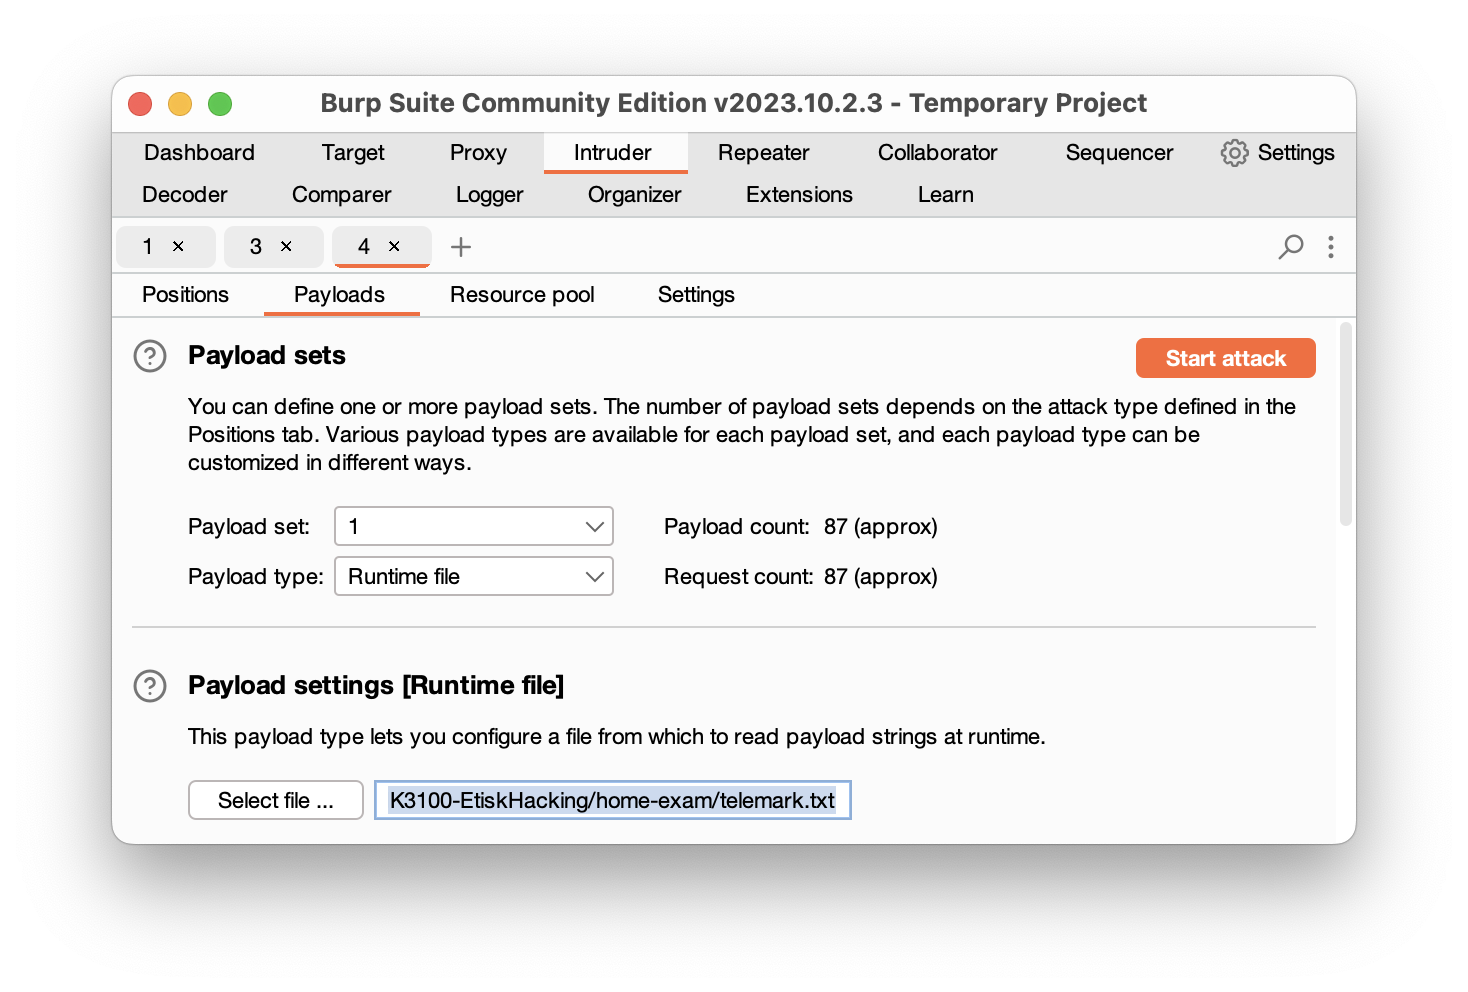
\includegraphics[width=15cm]{img/Web hacking/Arenabook/Skjermbilde 2023-10-26 kl. 14.54.29.png}
\end{center}

After the attack was done I searched through the results and found the following page:

\begin{center}
    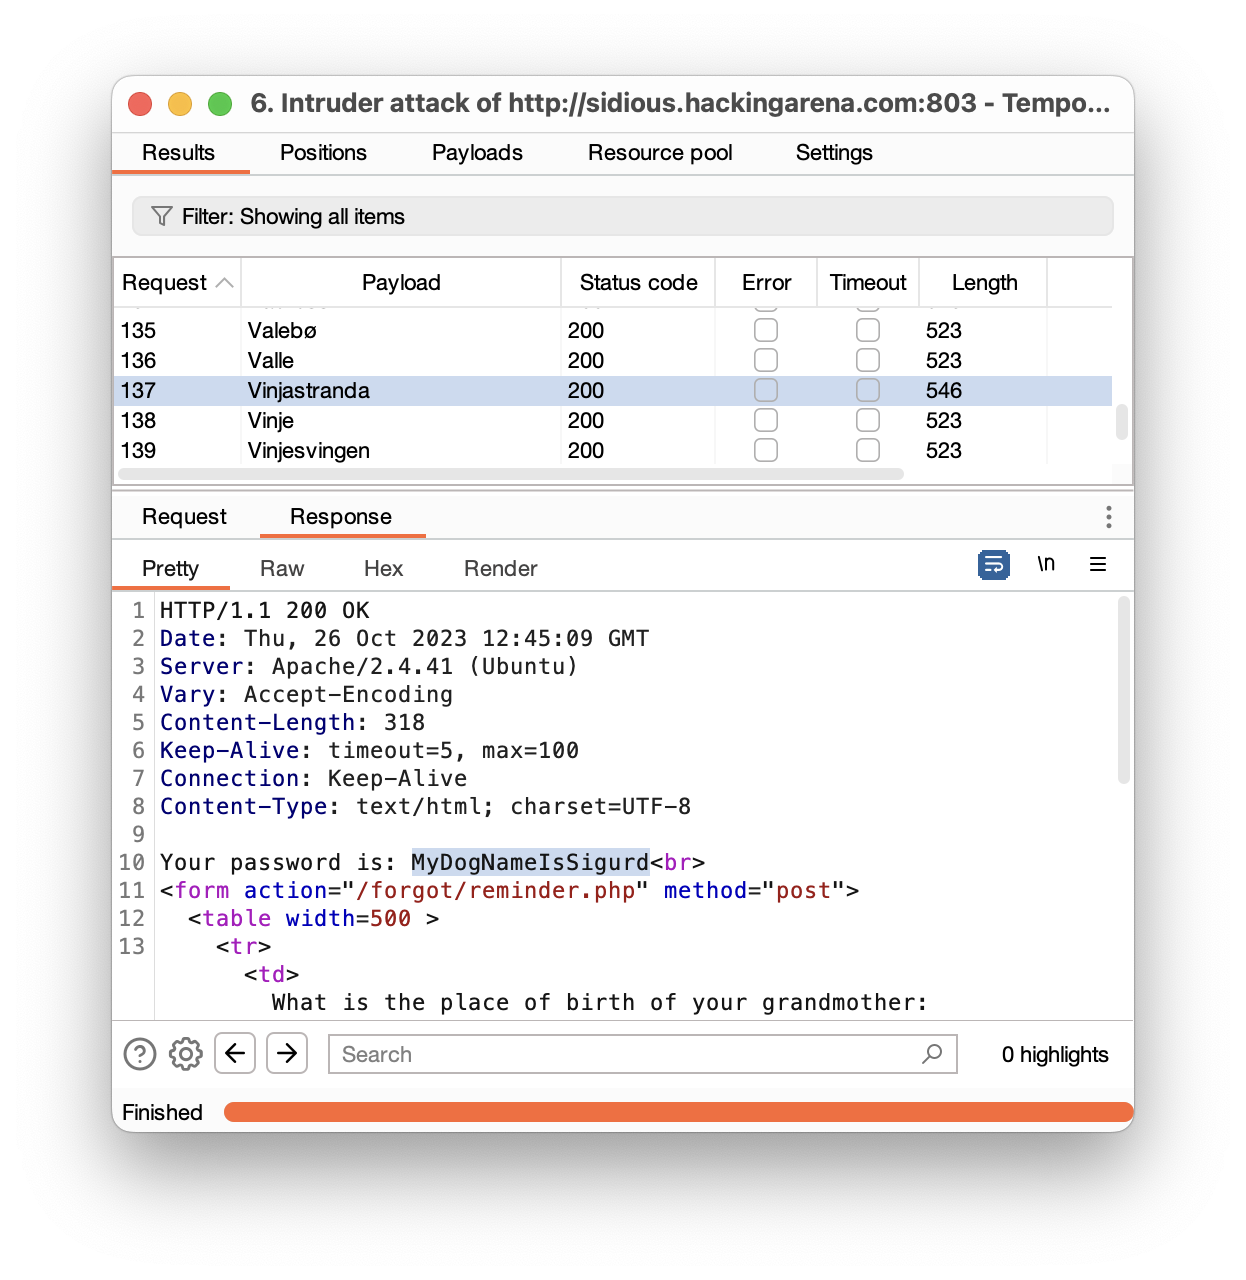
\includegraphics[width=13cm]{img/Web hacking/Arenabook/Skjermbilde 2023-10-26 kl. 14.55.08.png}
\end{center}

Sandras grandmother was born in \texttt{Vinjastranda}, and her password was \texttt{MyDogNameIsSigurd}. Using the password I could log in to Sandras account and get the flag.

\begin{center}
    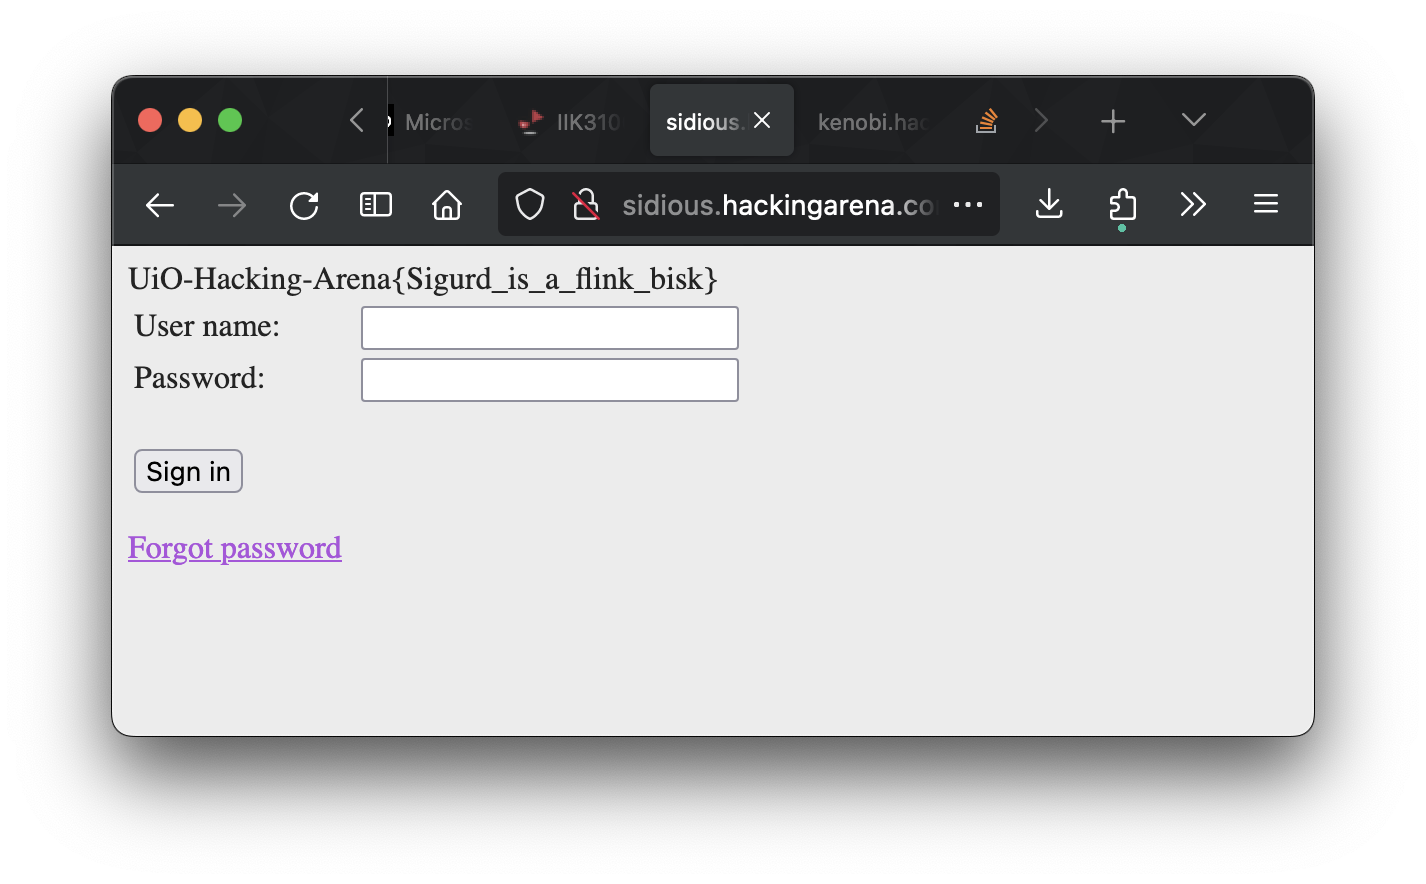
\includegraphics[width=12cm]{img/Web hacking/Arenabook/Skjermbilde 2023-10-26 kl. 14.55.36.png}
\end{center}
\section*{Total points: 710p}
\addcontentsline{toc}{section}{Total points: 710p}

% \printbibliography[heading=bibintoc] % LAGER BIBLIOGRAFI
\end{document}
